\documentclass[]{cwru}
\usepackage[acronym,shortcuts,nonumberlist]{glossaries}
\usepackage[toc,title]{appendix}
\usepackage{graphicx}
\usepackage{siunitx}
\usepackage{subcaption}
\usepackage[rightcaption]{sidecap} % Change if double-sided layout
\sidecaptionvpos{figure}{c}
\usepackage{color}
\usepackage{colortbl}
\usepackage{multirow}
\usepackage{longtable}
\usepackage{rotating}
\usepackage{array}
\usepackage{amsopn}
\usepackage{amssymb}
%\usepackage{hyperref}
\usepackage{amsthm}
\usepackage{amsmath}
\usepackage{mathrsfs}
%\usepackage{natbib}
\usepackage[square,sort,comma,numbers]{natbib}
\usepackage{complexity}
\usepackage{hyperref}
\usepackage[all]{hypcap}
\usepackage{epigraph}
\usepackage{algorithm}
\usepackage[noend]{algpseudocode}
%\usepackage{multipleinstance}
\usepackage{verbatim}
\usepackage{chronosys}
\DeclareMathOperator*{\argmin}{arg\,min}
\DeclareMathOperator{\atantwo}{atan2}
\MakeRobust{\Call}
\allowdisplaybreaks
\usepackage{tikz}
\usepackage{tkz-euclide}
\usetkzobj{all}
\usetikzlibrary{positioning,shapes.geometric,arrows,fit}
%\usetikzlibrary{bayesnet}
\tikzstyle{startstop} = [rectangle, rounded corners, minimum width=3cm, minimum height=1cm, text width=3cm, text badly centered, draw=black]
\tikzstyle{decision} = [diamond, aspect=2, minimum width=3cm, minimum height=1cm, text width=3cm, text badly centered, draw=black, inner sep=0pt]
\tikzstyle{sdecision} = [diamond, aspect=1.5, minimum width=3cm, minimum height=1cm, text width=3.5cm, text badly centered, draw=black, inner sep=0pt]
\tikzstyle{flowarrow} = [thick,->,>=stealth]
\tikzstyle{flowarrow} = [thick,->,>=stealth]
 
\tikzstyle{model} = [rectangle, rounded corners, minimum width=3cm, minimum height=1cm, text width=6cm, text badly centered, draw=black]
\tikzstyle{contribution} = [rectangle, minimum width=3cm, minimum height=1cm, text width=3cm, text badly centered, draw=black]

\definecolor{positivecolor}{RGB}{0,0,139}
\definecolor{negativecolor}{RGB}{139,0,0}
\definecolor{lightgray}{RGB}{215,215,215}
\newunicodechar{′}{\textprime}

\def\checkmark{\tikz\fill[scale=0.4](0,.35) -- (.25,0) -- (1,.7) -- (.25,.15) -- cycle;}
\newcolumntype{C}[1]{>{\centering\let\newline\\\arraybackslash\hspace{0pt}}m{#1}}

\setlength\epigraphwidth{10cm}
\setlength\epigraphrule{0pt}

\setlength\LTcapwidth{\textwidth}

\definecolor{highlight}{rgb}{0.8,0.8,0.8}
\newcolumntype{g}{>{\columncolor{highlight}}c}
\newlength{\oldtabcolsep}
\newlength{\tabcaptionsep}
\setlength{\tabcaptionsep}{10pt}

\hypersetup{pdfborder=0 0 0,pdfview=FitH}
\fancyhead[LO,RE]{}% Remove section names from header

\renewcommand*{\acronymname}{List of Acronyms}
\renewcommand{\chapterautorefname}{Chapter}
\renewcommand{\sectionautorefname}{Section}
\renewcommand{\subsectionautorefname}{Section}
\newcommand{\Appendixautorefname}{Appendix}
% begin appendix autoref patch [\autoref subsections in appendix](http://tex.stackexchange.com/questions/149807/autoref-subsections-in-appendix)
\usepackage{etoolbox}
\makeatletter
\patchcmd{\hyper@makecurrent}{%
    \ifx\Hy@param\Hy@chapterstring
        \let\Hy@param\Hy@chapapp
    \fi
}{%
    \iftoggle{inappendix}{%true-branch
        % list the names of all sectioning counters here
        \@checkappendixparam{chapter}%
        \@checkappendixparam{section}%
        \@checkappendixparam{subsection}%
        \@checkappendixparam{subsubsection}%
        \@checkappendixparam{paragraph}%
        \@checkappendixparam{subparagraph}%
    }{}%
}{}{\errmessage{failed to patch}}

\newcommand*{\@checkappendixparam}[1]{%
    \def\@checkappendixparamtmp{#1}%
    \ifx\Hy@param\@checkappendixparamtmp
        \let\Hy@param\Hy@appendixstring
    \fi
}
\makeatletter

\newtoggle{inappendix}
\togglefalse{inappendix}
% end appendix autoref patch
\newcommand{\thesisstatement}[1]{\emph{#1}}
\newcommand{\mypar}[2]{\textbf{#1 (#2).}}
\DeclareMathOperator{\sign}{sign}
%% =================
%% Title Page Setup
%% =================

\makeatletter

\title{Interactive Causal Feature Selection with Prior Knowledge}
\author{Helen Zhao}
\date{May 2019}
\degree{Master of Science}
\doctype{dissertation}
\department{Electrical Engineering and Computer Science}
\defensedate{March 25, 2019}

\begin{document}

\advisor{Dr.\ Soumya Ray}
\committee{Dr. Xusheng Xiao}
\committee{Dr. Michael Lewicki}
\committee{Dr. Andy Podgurski}


\maketitle
\makeapprovalsheet

\frontmatter
\tableofcontents

\cleardoublepage
\phantomsection
\addcontentsline{toc}{chapter}{List of Tables}
\listoftables

\cleardoublepage
\phantomsection
\addcontentsline{toc}{chapter}{List of Figures}
\listoffigures

%\begin{acknowledgments}

%\end{acknowledgments}

\begin{abstract}
Interactive machine learning (IML) uses visual analytics to leverage human intelligence while using machine learning methods. This is a natural way to integrate expert knowledge into the learning process. Feature selection, a critical step in classification that uncovers informative feature sets, is a natural candidate for IML. Domain experts are often knowledgeable about feature semantics, relevance to the classification task, causal relationships between features; however, automated algorithms may impose limits on how to use such information. We hypothesize that a human-machine collaborative approach to feature selection that incorporates human prior knowledge will yield high performing and transparent classifiers. We develop a novel visual analytics platform for interactive feature selection that allows domain experts to visually express background knowledge about feature relevance and causal interaction. Then they dynamically, iteratively explore the feature space to uncover and compare predictive feature sets that are consistent with their prior knowledge. We evaluate our approach through user studies. Our study showed that our system enabled participants to efficiently and effectively express prior knowledge, explore the feature space, and identify patterns in the dataset. Participants found the system intuitive and easy to use. Participants who were able to utilize previously expressed prior knowledge are able to more efficiently explore the feature set space and were better able to explain the behavior of the learned classifiers. 

\end{abstract}

\mainmatter

\chapter{Introduction}
In machine learning, classification is the process of creating a model that maps the input data \(X=[x_1, x_2, ..., x_N]\) to output label \(y\). Classification algorithms are given training examples described by features \(X=[x_1, x_2, ..., x_N]\), which are measurements or observations of characteristics of the examples, and a target label \(y\), which is the variable to be predicted. The number of features can range from tens to hundreds depending on the problem domain. Not every feature provides information about the target, so instead a subset of informative features is used to create the model. Feature selection is the process of selecting the features to create the model and is an important step in the classification process. Feature selection improves prediction performance by removing irrelevant or noisy features, prevents overfitting to training examples, reduces computational cost of training, and identifies relevant features. Moreover, reducing number of features also reduces the amount of data collection and preparation because less training examples is required to create a generalizable model.\cite{ReviewOfFS,  IntroToFS}.

Feature selection directly effects the created model. Poor sets of features results in poor performing models. Selecting a set of informative features is a difficult problem. Exhaustive search of the feature subspace is costly and impractical. An exhaustive search for the optimal feature set of size \(k\), \(k < N\) would explore \(N\choose k\) possible feature sets. If the size of the feature set is also optimized, then there are \(2^N\) possible combinations of features. The number of combinations grows exponentially with dimensionality which makes the search for the optimal feature set NP-hard \cite{IntroToFS}.

While uncovering causal relationships between features is not required for finding predictive features, feature selection can benefit from the integration of causal discovery. Although conventional feature selection algorithms select features based on their effectiveness at predicting the target label, they may select features that are results of the experimental side effects rather than a property of the studied system \cite{CausalFS}. Furthermore, the user can build more understandable models that explain the underlying data generation mechanism by being aware of the cause and effect relationships in the data. 

\begin{figure}[h]
\centering
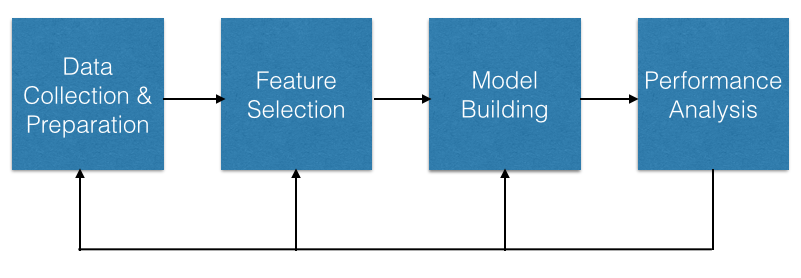
\includegraphics[width=1\textwidth]{MLflow}
\caption{ \textbf{Machine Learning Process.} Machine learning is typically an iterative approach. Many iterations are needed to create a model. The expert modifies inputs to the algorithm using the analysis of the current model's performance. From performance analysis, our system returns the user to feature selection step and allows the user to test a new feature set using newly acquired insights. }\label{fig:MLflow}
\end{figure}

We propose an interactive, iterative framework for feature selection that incorporates background knowledge. Machine learning is typically an iterative process consisting of data collection and preparation, feature selection, model creation, and performance analysis. In standard machine learning procedures, algorithms are often fully automated and domain expert’s contributions ends after collecting and preparing the data. Although the user can control the behavior of standard algorithms by tweaking input parameters, such as the depth of a decision tree, it is difficult to find the optimal parameter settings, which often change for different problem domains. As a result, the user has limited control and understanding of the algorithm. As opposed to automated machine learning, interactive machine learning engages user in generating the model. Furthermore, interactive machine learning is a natural method for integrating background knowledge. Interactions and interfaces can be designed to support efficient and effective communication between the expert and the algorithm. Moreover, an interactive approach can also account for the iterative aspect of model creation. 

We hypothesize that collaborative feature selection between the practitioner and learning algorithm will yield in a more understandable and higher performing model than non interactive feature selection techniques. Although computers are superior than humans at efficiently performing vast amounts of calculations, machine learning algorithms can still benefit from collaborating with humans. Domain experts have a rich understanding of the problem domain and the semantics of the input data, and interactive machine learning is a natural method for integrating prior knowledge that is difficult to express and encode in algorithms. Many of the classification datasets in the UCI repository have characteristics that can be explained to a human or understood by experts but are difficult to encode in a classification algorithm. 

To the computer, the characteristics are just rows and columns of numbers. The expert who often is involved in data collection and processing understands how the data values maps to real world situations and the meaning of the feature. An example is the meaning of the features in the breast cancer dataset built by Dr. Wolberg, a medical expert at the University of Wisconsin Hospitals. In the breast cancer data set, the feature clump thickness ranges from 1 to 10 and describes the extent to which the epithelial tissues lining the outer surface of the organ were one layered (1) or multilayers (10). Experts in breast cancer can map a value to its meaning in reality, understand the feature's relationship to other features and the possible implication a value has on the presence of breast cancer. Involving human in the feature selection process enables the user to interpret the model behavior and the predictions of individual examples.

Visual analytics is the use of interactive visual representations of data to gain insights into large, complex datasets. and can be used to help users efficiently gain insights into the data and the machine learning techniques. Visualizations is important tools for expressing information. Visual elements such as charts, maps, and graphs are often used to perform data analysis and gain insights about complex, high dimensional data that are difficult to manually analyze. Visualizations translate raw data into useful information that users are able to visually extract. For example, causal relationships is more easily communicated visually and are represented as directed acyclic graphs (DAG) where nodes represent features and direct edges represent cause and effect relationships as seen in figure \ref{CBN}. An integration of visual analytics techniques and classification methods can improve the the performance and transparency of the model created. Moreover, visual analytics can be used to facilitating communication and collaboration between the practitioner and the algorithm. Visualization can be used by both humans and machine to communicate information to each other in an efficient and effective manner. For example, users can interact with visuals to encode their soft knowledge in the visual system which can then translated the encoding to the algorithm. The algorithms uses the information provided by the user to perform calculations and can report the results to the user through visualizations.

In this thesis, we propose to perform feature selection as a collaborative effort between the user and the computer. For that purpose, we integrated feature selection techniques and visual analytics into a interactive visualization system. We devised a workflow that accumulates prior knowledge and incorporates the information into the exploration of possible feature sets. The user first encodes their background knowledge using interactive visualizations. The system expresses features visually, allows the user to interactively explore feature sets and build models from the feature set. Prior knowledge is incorporated in the exploration of feature space by calculating how consistent the feature subset is to the information previously provided by the user. Moreover, we incorporate performance analysis and design our system to account for the iterative nature of machine learning. The expert can create models and use their performance analysis to gain insights on other possible predictive feature sets; they can create many models and compare and contrast their performance and feature sets. We also present an evaluation of the effectiveness of the system in performing feature selection.

\indent Our contributions are a collaborative framework for feature selection that includes:
\begin{itemize}
  \item an interactive visualization for users to encode their prior knowledge about feature's relevancy to the target and a ranking of feature importance.
  \item a feature selection workflow that integrates causal discovery into the feature selection process and allows users to analyze causal networks and express their prior knowledge of causal interaction between features.
  \item an interactive visualization that enable users to dynamically explore possible feature sets and also communicates how consistent the feature set is to the prior information encoded.
  \item a performance analysis step that enable users to analyze the performance of models and compare the performance of models created from different feature sets.
\end{itemize}

Chapter 2 will provide necessary background knowledge on feature selection, visualization, and describe algorithms used in the thesis. It will also describe previously proposed and implemented visualization systems for machine learning. Chapter 3 describes the design and purpose of the interactive feature selection system. Chapter 4 describes the the design of the user study for evaluating the effectiveness and usefulness of the visual system. Chapter 5 presents the results of the evaluation study. Lastly, Chapter 6 presents conclusions, challenges and directions for future work.


\cleardoublepage
\chapter{Background and Related Work}
\indent This chapter introduces the context and background for this thesis.
\section{Interpretability}
\indent Machine learning practitioners have a wide palette of methods and tools. With advances in methodologies, practitioners are able to create high performing models for increasingly complex tasks and problems. A variety of models are produced from the diversity of machine learning algorithms and techniques. However, many models with impressively high performances are treated as black boxes - the information and reasons why they arrived at a prediction or decision is not transparent. An example of non-transparency is AlphaGo, a deep learner for playing the game Go, whose decisions for making moves in are unclear. \cite{InterpretDLModels}. The practicality of machine learning systems depends on whether humans can interpret and extract knowledge from the model and trust its predictions \cite{MakeMLInterpretable}. No matter how complexity or high performing the model is, if the system cannot explain its reasoning in a way the human can understand, humans can not act on the system’s decisions.

\indent In machine learning, a system is interpretable if is able to explain in understandable terms to humans. Researchers recognize the importance of interpretability and the amount of research in interpretable machine learning has grown along with surge in deployment of machine learning systems in all domains \citet{RigorousIntretable}. Doshi-Velez and Kim argue that interpretability is needed because problems are fundamentally under-specified. For example, an algorithm’s objective function may be slightly off from the target function and it is computationally or logically unfeasible to enumerate and test all possible inputs to a model. Therefore, the evaluation of an algorithm based on its optimization of the objective function is incomplete. Moreover, the ability to interpret the model is important for debugging, pinpointing the source of error and improve on the current model, and establish trust in the model. 
\section{Feature Selection}
\subsection{Problem Definition}
\indent Classification is the process of categorizing data points into a given set of categories. The category is also known as the target or the class label. The classification task is to approximate a mapping function from the input \(X=[x_1, x_2, ..., x_N]\) to the output class label \(y\) and creates a model that predicts the class label of a data point represented by a set of inputs also known as a feature vector. Features are measurable properties or characteristics that will help predict the target class. An example of a classification problem is predicting whether an email is spam or not spam. The target classes are spam and not spam, and features describing the emails can be word count, frequency of words, location email sent from, etc. 

\indent In supervised learning, we are provided with \(N\) features \(X=[x_1, x_2, ..., x_N]\), the target variable \(y\), and training examples drawn from the probability distribution of \(X\) and \(y\). Features are measurements or observations of properties and characteristics. The size of the feature vector varies from tens to hundreds or even more. The feature selection is the problem of selecting a subset of features in \(X\) to create a mapping to the target output \(y\) that will maximize the objective which is often the prediction performance of the constructed model on future examples.

\subsection{Introduction}
\indent Feature selection is performed before constructing a prediction model for many important reasons. Feature selection can help improve performance by removing irrelevant or noisy features and prevent overfitting to the training examples. Other benefits of feature selection include reduction in computational cost of training models and identification of features relevant or related to the target variable. Also less data is needed to be collected and processed because more training examples are required to create a generalizable model as the number of features increase. Moreover, a smaller feature set creates simpler models that are more easily interpreted by humans and explanatory of the underlying data generation mechanisms.  

\section{Common Feature Selection Strategies}
\indent An exhaustive search of an optimal feature set of size \(k\), \(k < N\) would explore \(N\choose k\) possible feature sets. If the size of the feature set is also optimized, then there is \(2^N\) possible combinations of features. The number of combinations grows exponentially with dimensionality making the search for the optimal feature set a NP-hard problem. Exhaustive search of the feature subspace is costly and impractical. Conventional feature selection strategies are composed of a search algorithm, an objective function to evaluate the feature subset, and a stopping criterion to stop the search. The search algorithm is independent of the evaluation function.

Two techniques for searching through the features subspace are feature ranking and subset search. In the feature ranking methods, features are ranked based on a merit value such as information content, entropy, relevance, etc. and the top \(k\) candidates are selected. The downside is that redundant and irrelevant features are not always removed. In subset search methods, the search process and elementary operations such as addition or removal of a feature to the current features subset are guided by the value of the objective function. The exploration can be computationally expensive with large feature sets and possible combination of features. 

The three main categories for feature selection approaches are filter, wrapper, and embedded. 
\subsection{Filters}
\indent Filters use the feature ranking technique to evaluate individual features or the feature subset based on measures of information, distance, consistency, similarity, and statistical measure \cite{ReviewOfFS}. Evaluation metrics are independent of the performance of the classifier. Filters can be easily used for most classifiers and useful for very high dimensional data because of their fast computation in comparison to the other two methods. However, the selected subset of features does not necessary build the best performing classifier because the evaluation metric may not relate to the performance of the classifier. A popular filter method is a Correlation based Feature Selection algorithm (CFS) proposed by Hall in 1996 \cite{FSAlgo} build on the heuristic that the features highly correlated with the target variable and uncorrelated with each other are good features for the problem. 

\subsection{Wrapper}
\indent Wrapper methods utilized the subset search technique. Since an exhaustive search for the optimal feature set is NP-hard, wrapper methods are suboptimal searches and some greedy method are on computational scale of \(O(N^2)\) \cite{Clopinet}. Forward selection start with an empty set and add features, while backward elimination start with a feature set and subsequently remove features. One example of wrapper method is forward feature selection, a greedy algorithm that starts with an empty feature set and iteratively adds the feature that would most improve an objective function. The classifier’s prediction performance is the common objective function guiding the search to the feature subset that would maximize the classifier’s performance. Wrapper methods can be used with most learning algorithm because the classifier is treated as a black box, but the resulting feature subset is optimal for the specific learning algorithm. A downside of wrapper methods is that the search space grows with the number of features and is computationally expensive because the classifier has to be reevaluated for every new subset of features and becomes unfeasible for large data sets and more computationally expensive learning algorithms. 
\subsection{Embedded and Hybrid}
Embedded methods incorporate or embed feature selection as a part of the learning algorithm. Various variants of decision tree algorithms, such as CART and random forest, are embedded methods. Hybrid methods combine the desired properties of filter and wrapper methods. A filter is first used to reduce the feature space and then a wrapper method is used to find the best feature subset.  

\section{Causal Feature Selection}
\indent Conventional feature selection algorithms in machine learning literature do not uncover causal relationships among features and between feature and target. Although discovering mechanisms not required for finding good predictors, awareness of cause and effect relationships can support in building more transparent model. Moreover by selecting features based on their effectiveness at predicting the target variable, feature selection algorithms may select feature that are the results of experimental side effects rather than a property of the studied system. The causal information provided by the selected features will help interpret the model’s predictions and make them more trustworthy. 

\indent Feature selection can benefit from causal discovery by revealing relevant features and increasing understanding of the data structure. The goal for the causal discovery problem is to discovery the causal relationship between features for a set of \(N\) input features \(X = [x_1, x_2, ..., x_n]\). The target variable is not singled out and any variable can be the target. 

\subsection{Causal Bayesian networks}
\indent Simple models of cause and effect relationship is based on Bayesian networks which aids in the understanding causality. Causal Bayesian networks is framework for representing the causal relationships for a set of random variables \(X = [x_1, x_2, ..., x_n]\) in the structure of a network. A Bayesian network is a directed acyclic graph (DAG) where each node map one to one to a variable in the set of variables \(X\). The Markov condition of Bayesian networks require every node to be conditionally independent of non descendent nodes given its parent node. A causal Bayesian networks is a Bayesian network where directed edges represent the relationship between variables. For all \(x_i\) and \(x_j\) in X, if there is a directed edge from \(x_i\) to \(x_j\), feature \(x_i\) is a direct cause of feature \(x_j\), then A directed path between two nodes indicates a causal relationship. Causal Bayesian network is a map of the dependencies and independencies of X. 

\subsection{d-separation}
Node \(x_i\) is d-separated from \(x_j\) by Z if Z is a set of node that blocks every path between \(x_i\) and \(x_j\). If \(x_i\) and \(x_j\) is not d-separated by C, then they are d-connected. In a causal Bayesian network, two nodes \(x_i\) and \(x_j\) is d-separated by Z if and only if \(x_i\) is conditionally independent of \(x_j\) given Z. \(x_i\) and \(x_j\) are d-connected \(iff\) they are conditionally dependent \cite{Clopinet}. 

\subsection{Markov blanket}
\indent The Markov blanket in a Bayesian network is the set of features that separates a given feature from the rest of the features in the graph. The Markov blanket is composed of direct causes (parents), direct effects (children), and direct causes of direct effects (spouses). Once all the direct causes of the target are known, indirect causes do not provide any additional information since their effect on the target is through a direct cause and captured in the direct cause. Although the children of the target are predictive of the target, knowing all the other causes of the target’s children (spouses) can help explain the amount of effect the target has on the children. The direct causes along with the direct effects of the direct causes enhance each others predictive power. Researchers has suggested that the Markov blanket for the target variable is an important concept for the feature selection problem \cite{MBforCL}. Feature relevant can be be described in relation to the Bayesian network. For any feature \(Y\), a irrelevant feature is disconnected from Y in the network. Features in the Markov blanket of \(Y\), \(MB(Y)\) are strongly relevant features. Features that are not in \(MB(Y)\) but have a directed path to Y are weakly relevant features \cite{Clopinet}. 

\subsection{Causal discovery algorithms}

\indent Learning causal relationships from observation data is a heavily researched area. The two parts of learning a Bayesian network are learning the structure of the graph G and the probability distribution of the variables. Algorithms for discovering the Markov Blanket that attempts to induce the complete causal Bayesian network does not scale with the increase in features. HITON is a more efficient method proposed for discovering Markov blanket \cite{HITON}. HITON first identifies the children and parents of the target. Then then identifies the children of the parent and the parent of the children of the target. Next, a wrapper method is used to search through the possible feature subset and return feature subset that resulted in the best performing classifier. 

\subsection{Greedy Equivalence Search}
The Bayesian network learning problem is to identify a DAG that fits the observed data \(D\) based on an objective function. The Greedy Equivalence Search (GES) algorithm \cite{GES} identifies an optimal structure and can be used to learn a causal network that fits the observed input data. For two DAGs \(H\) and \(G\), \(H\) is an independent map of \(G\) if the independence between variables implied by the structure of \(H\) is also implied by the structure of \(G\). For an independence map H of G, there exist a finite sequence of edge modification that can be applied to G such that after each edge modification H is still an independence map of G and at the end of the sequence G = H. H, G, and the intermediate DAGs G' are a part of the same equivalence class and are said to be equivalent. Meek proposed a two phase greedy algorithm that optimizes a Bayesian scoring function to find the network structure to map the observed data distribution. The algorithm starts with the equivalence class of DAGs that has no dependencies in the structure. In the first phase, edges are greedily added dependencies by considering all single edge addition that can be made to all the DAGs in the current equivalence class. After the algorithm stops at a local maximum, in the second phase, all single edge removals that can be made to all the DAGs in the current equivalence class are considered. The algorithm outputs the local maximum structure at the end of the second phase. Chickering \cite{GES} proved Meek's Conjecture and provided an implementation of GES. Later in the paper, we will be using a causal discovery tool \cite{Pycausal} implemented by the Center of Causal Discovery that performs GES.

\section{Visualization}
\subsection{Visual Analysis}
\indent Machine learning problems often use complex, multivariate data sets that are difficult to explore and gain insights from. When calculating aggregated statistical measures from large data sets, information is lost from oversimplification and misleading information is a common side effect. Visualization is one of the most relevant knowledge extraction method and can help translate raw data into useful information. Visualization of data helps communicates information and enhance people’s understanding of the data. Visual elements such as charts, graphs, maps can people visually and more efficiently identify trends, outliers, and patterns in the data. 

\indent Visual analytic is the combination of visualizations, human factors, and data analysis and the study of analyzing complex data set supported by interactive graphical and visual interfaces.
Although humans are significantly slower than computers, humans have soft knowledge that can not be expressed as inputs to an algorithm. While computers can performance fast calculations with numbers, the inputted data is all they know. For example, for machine learning classification models, the inputs are examples described by a set of features expressed in a table where rows are examples and columns are features. While the algorithm performs and optimizes calculations with the tabular data, the human has knowledge of the mapping from data values to situations in the real world and understand the rich information behind each feature. Furthermore, humans building the models often have a rich knowledge of the problem background and can catch spot mistakes the machines are making or the incorrect conclusions they may arrive at. Humans are also the ones judging whether the model is sensible in the end. Visual analytic is able to combine the computational and processing power of computers with the high visual processing power of humans and their prior knowledge of the problem. By allowing humans to interact with model, incorporate their prior knowledge, and analyze complex model through visual representations, they build a greater understanding of models and increase the trust of its predictions. 

\subsection{Visualization in Machine Learning}
\indent Visual analytic techniques and tools have been proposed and implemented for every step of the machine learning training process to support users in understanding, diagnosing, and improving models. Visualization systems have been created for specific machine learning models such as decision trees and neural networks and for specific domains such as natural language processing. For example, Stef van den Elzen created BaobabView \cite{BaobabView}, an interactive visual system for the construction and analysis of decision trees that incorporates the expert and their prior knowledge, and Yosinski released a software tool to study large deep learning networks through visualizing every neuron in a trained network as it responds to an input image \cite{Yosinski}. Another technique proposed to explain and visualize local explanations, the model’s output for a single example, to establish trust in a model’s predication. Tamagnini implemented Rivelo \cite{Tamagnini}, an explanation interface for interacting and exploring instance level explanation, which is the set of features that explains the prediction of an example. 

\subsection{Performance Analysis}
\indent Other visual systems extract knowledge from the model’s output to allow the users to interact with the visuals of the model’s output to evaluate its performance and explore and understand the model’s predictions. An example of performance analysis systems is ModelTracker \cite{ModelTracker} which lays out examples horizontally from low to high scoring examples to convey overall performance and enables users to directly interact and inspect examples for debugging. Also, Alsallakh created a system for visualizing probabilistic classification data that lays out histograms of prediction scores for each class in a circle to form a confusion wheel \cite{}. 
\indent I had proposed a set of visual methods that can facilitate analysis of the performance of probabilistic classifiers. The methods were integrated into Stacks, an interactive visual analytics system. Prediction scores are shown at the class level using histogram plots. Users can hone in on mistakes by filtering out irrelevant instances. The distribution of prediction scores communicates how confident the classifier is at its prediction. Furthermore, Stacks also incorporated error analysis for assessing why examples may be falsely classified or received a low prediction score.

\subsection{Visualizing for Feature Selection}
\indent Dimensionality reduction is a common strategy for reducing high dimensionality algorithm and to visualize and analyze high dimensional data in one, two, or three dimensional space. For example, t-Distributed Stochastic Neighbor Embedding (t-SNE) is a dimensionality reduction technique and useful for visualizing high dimensional data sets. 

Non-traditional methods of applying dimensional reduction has been implemented and utilizes visualization. Guo in 2003 \cite{Guo} implemented an interactive feature selection approach that uses visuals to identify patterns and feature subspaces from the high dimensional space. Every pair of features is represented in colored matrix where the color codes for the pair wise similarity. The matrix is sorted to highlight interesting clusters in feature subsets, and users can choose a reduced set of features to display the input data. Fernstad and Johansson created an interactive dimensionality reduction system \cite{InteractiveDR}whose process is influenced by the user. The user chooses the metric and parameters that the system uses to select the most import features and then the reduced features are displayed in a parallel coordinate visual or scatterplot matrix. Moreover, INFUSE \cite{INFUSE} is an interactive feature selection system that ranks features by its predictive power calculated across various feature selection algorithms and classifiers and visualizes the ranking in a sorted list. Users can select features to create their own model and compare their custom model to the other established feature sets.

\section{Evaluating Visual Systems}
\cleardoublepage
\chapter{Interactive Feature Selection Design}
In this section, we outline the design goals of our system and describe the design of each component and interaction. The system's workflow for collaborative feature selection is derived from the analysis of feature selection techniques and ideas on how to incorporate humans into the techniques. We describe each step of the process and explain how each step supports collaborative feature selection. We also describe how the overall system supports iterative predictive modeling and how to compare different models.

\section{Design Goals}
The first design goal of the system is to facilitate collaboration between the user and machine at performing feature selection. The second design goal is to design interactions and visualizations that support efficient and effective communication. Lastly, the system is designed to establish and incorporate prior knowledge which would support the user at filtering features. Feature relevance and causal relationship are two types of prior knowledge that we identified and integrated into the system. The system is designed such that we can easily integrate another step in the workflow to capture other aspects of prior knowledge. 

\subsection{System Overview}
We devise a workflow for collaborative feature selection. The steps of the process are expressing feature importance, expressing causal relationships, exploring feature sets and creating a model, and analyzing and comparing model performances. We first acquire prior knowledge from the user and integrate that information into the rest of the workflow. The purpose of the first two steps, expressing feature importance and expressing causal relationships, is to acquire prior knowledge. In the next step, the user interactively explores the feature space and the system assesses how consistent the feature set is in relation to the previously provided information. Then a model is built using features manually filtered by the user. Lastly, the user evaluates and compares the performances of different models.

Separate interfaces and interactions are designed for each step. The steps are chronologically outlined at the top of the interface and the current step is highlighted. 

\section{Expressing Feature Importance}

\begin{figure}[!htbp]
\centering
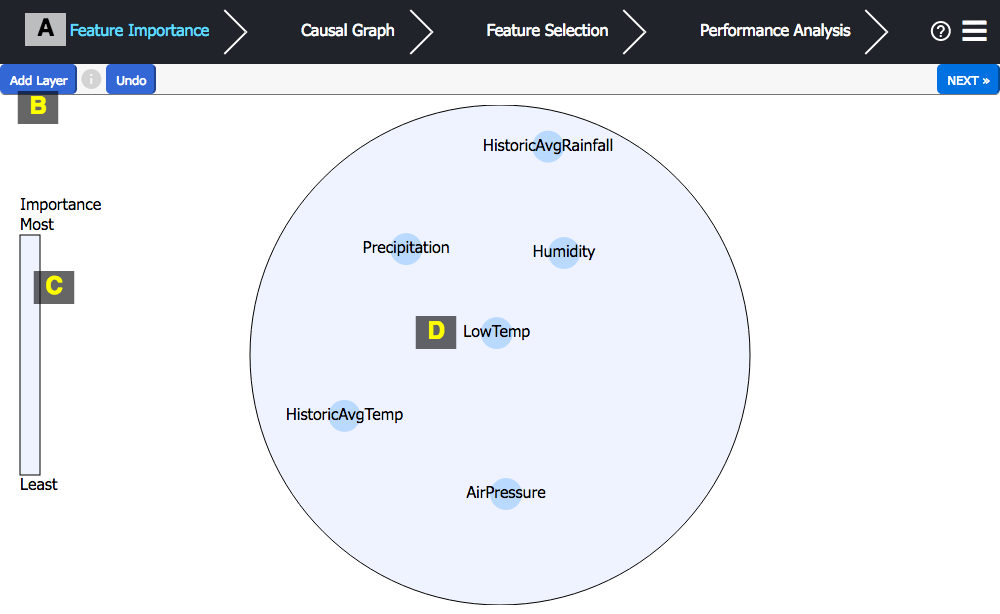
\includegraphics[width=1\textwidth]{InitialUserInterface}
\caption{\textbf{Initial User Interface for Expressing Feature Importance}. The classification task in the following figures is predicting tomorrow's weather conditions based on today's weather metrics. (A) The steps of the feature selection process are outlined horizontally at the top of the interface. (B) The user can click the 'Add Circle' button to create an additional inner circle that will represent a grouping of features with about the same level of importance. (C) A legend correlates the color of a circle to its relative level of importance. (D) Concentric circles are used to visually express the different levels of feature importance at predicting the target. }\label{fig:InitialUserInterface}
\end{figure}
 
\begin{figure}
    \centering
    \begin{minipage}{0.5\textwidth}
        \centering
        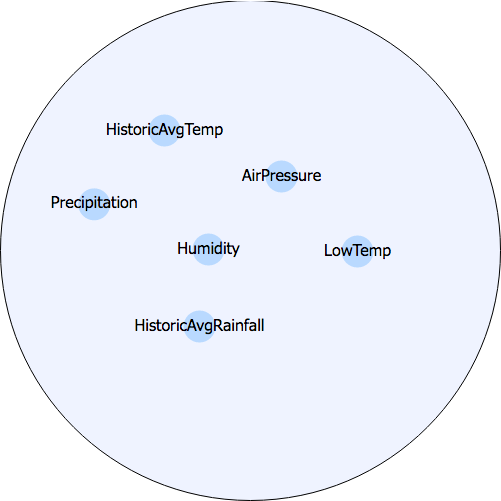
\includegraphics[width=0.825\textwidth]{FeatureImportance1}
    \end{minipage}\hfill
    \begin{minipage}{0.5\textwidth}
        \centering
        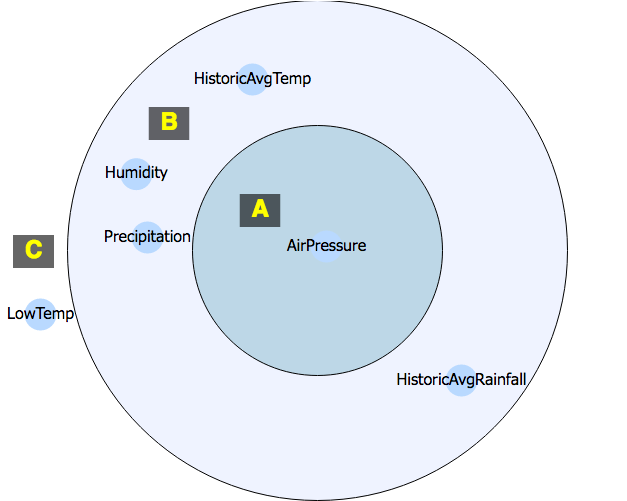
\includegraphics[width=1\textwidth]{FeatureImportance2Labeled}
    \end{minipage}
    \caption{\textbf{Express Feature Importance.} (Left) Initially, all features are grouped in the same circle to express that they are equally important at predicting the target (Right) (A) Air pressure is most relevant or important feature for predicting weather condition (B) The user does not know whether historical average temperature, humidity, precipitation, and historical rainfall are relevant to tomorrow's weather condition or the user does not think those features are as important as air pressure. (C) Today's recorded low temperature is not relevant to the classification task.}
    \label{fig:ExpressFeatureImportance}
\end{figure}

The user often has a rich knowledge of the problem background and feature semantics that the feature selection algorithms do not know about. The first step enables the user to visually express their prior knowledge about the importance or relevance of features at predicting the target label. The motivation is to integrate the user's prior knowledge as a criterion for filtering features. 

As shown in figure \ref{fig:InitialUserInterface}, the system represents features as labeled nodes and uses concentric circles to represent a ranking and grouping of importance. Features placed in the same circle are equally important. Initially, the system has no information about feature importance, and all features are grouped inside one large circle to represent that they are equally important at predicting the target label (figure \ref{fig:ExpressFeatureImportance}). If the user has no background information about which features may be relevant to the target, the user can move onto the next step without interacting with the visual. 

Otherwise, the user can interact with the visual to express which features are relevant, more relevant than others, or irrelevant. To express that a feature is more relevant than others, we distinguish the feature by placing it in a different group. We click the ``Add Circle" button to add an inner circle which represents a group of more relevant features. We leave the features that are either less relevant or we have no prior knowledge about in the outermost circle. In addition, we indicate a feature is irrelevant by moving it outside of the circles or groups as shown in figure \ref{fig:ExpressFeatureImportance}. 

Moreover, we can order features in terms of relevance. The user may have evidence that a feature may be predictive of the target, but the feature may not be as predictive or the user may not be as certain about its relevance compared to features in the innermost circle. To express this, the user can add another concentric circle and place features into the second most inner circle as shown in figure \ref{fig:FeatureImportance3}. Therefore, the groups of features also represent an ordering of feature importance. The user can continue to add inner circles to represent a group of features with the same level of importance and express a group's importance relative to the other groups. 

\begin{figure}[!htbp]
\centering
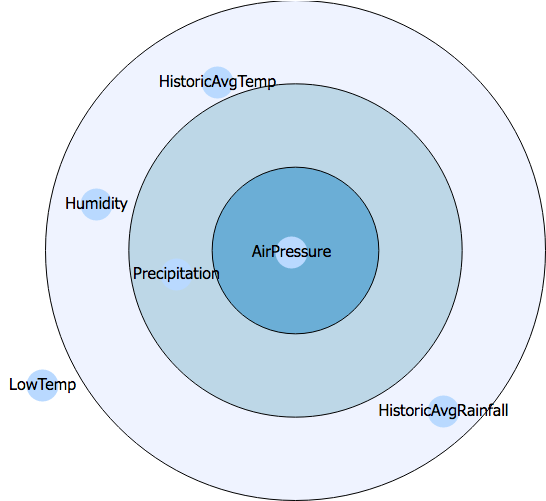
\includegraphics[width=0.65\textwidth]{FeatureImportance3}
\caption{\textbf{Ordering Feature Importance.} Air Pressure in the innermost circle is the most relevant feature. Precipitation in the second inner circle is more relevant than the features in the othermost circle but less relevant than air pressure.} \label{fig:FeatureImportance3}
\end{figure}

The interface is designed to help users visually translate their prior knowledge. The coloring of the concentric circles is a gradient. Humans are visually biased towards darker colors representing more. So the innermost circle is colored the darkest blue to represent the group with most relevance, while the outermost circle is the lightest blue to represent the group with the least relevance. Irrelevant features are placed in a white background, reinforcing that these features do not relate to the features in the colored circles. The gradient coloring of the concentric circles also corresponds to the ordering of feature relevance, and the color helps reaffirm the importance of features grouped in the circle.

When the user explores the feature space, the consistency of a feature set in relation to feature importance is quantified to help the user assess the feature set. The system treats the feature importance ordering and feature selection as rankings and measures consistency using rank loss. The feature importance visual can be translated to a ranking where more important features have higher ranks. The most important features in the innermost circle have the highest possible rank of 0. The immediate outer circle has a rank of 1; rank increments by one as we move towards outer circles, and features outside of the concentric circles are given the lowest rank. Feature selection can also be described as a ranking function, where selected features have the highest rank of 0 and not selected features have a rank of 1. The ranking function for feature selection, where $S$ is the set of selected features, is 
\begin{equation}
  f(x) =
    \begin{cases}
      0 & \text{if $x \in S$}\\
      1 & \text{otherwise}
    \end{cases}       
\end{equation}

Feature selections are converted to rankings and compared against the feature importance ranking. A list-wise approach is used to calculate the rank loss between the feature selection ranking function and feature importance rank list. 
\begin{equation}
\label{eqn:rankloss}
L(f; X, y) = \sum_{s=1}^{n-1}(-f(x_y(s)) + ln(\sum_{i=s}^{n}exp(f(x_y(i)))))
\end{equation}
where \(X = {x_1,..., x_n}\) is the feature vector to be ranked and \(y\) is the feature importance ranking list \cite{RankLoss}. 
A feature set that minimizes rank loss is more consistent with the feature importance ranking. However, noted that all the features are ranked 0 by default when the user does not have prior knowledge about relevance; therefore, \(L\) equals 0 for all possible selected feature sets. Although in this case, the rank loss does not help discover predictive feature sets, the system is designed to be used for classification problems where the user has prior knowledge to contribute. 

\section{Expressing Causal Relationship}
\begin{figure}[!htbp]
\centering
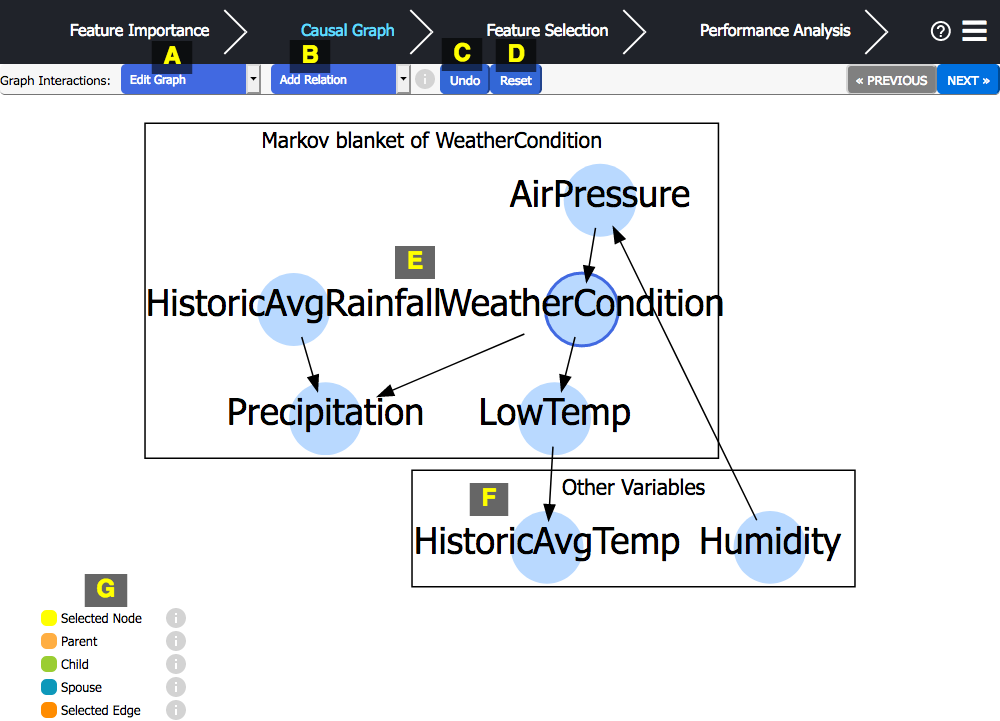
\includegraphics[width=1\textwidth]{LabeledCGInterface}
\caption{\textbf{Expressing Causal Relationship Interface.}  (A) User can select how to interact with the graph. The two graph interaction options are ``Highlight Selected" and ``Edit Graph". (B) The user can choose to highlight the selected feature's Markov blanket or its paths to/from the target. The user can edit the graph by adding an edge, removing an edge, reversing an edge, or removing a feature. (C) The user can undo graph edits. (D) The user can reset the graph to the original. (E) The interface shows a possible causal network fitting the weather condition dataset. The target variable, weather condition, and its Markov blanket features are outlined to highlight a predictive feature set based on causality. (F) The other features are grouped in a different subgraph. The edges between the subgraphs show which non-Markov blanket features are affected by or effect Markov blanket features. For example, the non-Markov blanket feature, historical average temperature is affected by low temperature. (G) The color of the highlighted features indicates their relationship to the selected feature. Initially, no feature is selected.} \label{fig:LabelCGInterface}
\end{figure}

As described in section \ref{CausalFSSubsection}, research has shown that feature selection techniques benefit from the integration of causality. In the second step, the system constructs a causal network that fits the dataset and also represents prior knowledge the user may have about cause and effect relationships in the dataset. We include information about feature importance in the causal discovery algorithm. Moreover, we seek help from the user at modifying the graph. The motivation for the second step is to interactively construct a graph that represents possible causal relationships and also is reflective of the user's prior knowledge. Causality is then incorporated as a filter criterion for feature selection.

Since causal discovery is not the primary contribution of this project, we designed the system to be agnostic to causal discovery algorithm. We integrate a causal discovery library, PyCausal, implemented by the Center of Causal Discovery rather than implement an algorithm ourselves. We use Greedy Equivalence Search (GES), a causal discovery algorithm described in subsection \ref{GESSubsection}, to build an initial causal network fitting the observed data. We can replace GES with another causal discovery algorithm without affecting the interface and functionalities.

We designed the system to build upon previously expressed prior information. For example, we incorporate feature importance as prior to the network. We impose direct dependencies between highly relevant features and the target variable. The algorithm will output a network containing direct edges between the highly relevant features and target. The direction of dependence is not imposed since we assume both direct cause or direct effect are highly relevant. Similarly, we impose independencies between the irrelevant features and target variable, and so irrelevant features do not directly connect to the target in the output network. The user is allowed to go back and modify feature importance. Since the causal graph depends on the information provided at the feature importance step, the causal graph is rebuilt when feature importance changes.

The causal relationships discovered by the algorithm are represented in a Bayesian network described in section \ref{CBN}. The graph is modified to help users visually identify important information. The Bayesian network is divided into two subgraphs; features are divided into those that are Markov blanket features of the target and those that are not. As shown in figure \ref{fig:LabelCGInterface}, the subgraphs are outlined to highlight the Markov blanket features of the target. Edges between Markov blanket features and edges between non-Markov blanket features are confided in their respective subgraphs, while edges between Markov blanket features and non-Markov blanket features appear between the subgraphs. The purpose of this design is to help the user identify features that influence the target through their influence on the target's Markov blanket features. 

\subsection{Highlighting Information in the Causal Network}
We designed the interactions to help users extract visual information. First, the user can click on a feature to highlight its Markov blanket and identify features that are directly related to the selected feature. As shown in figure \ref{fig:CausalGraphs}, the parents, children, and spouses are highlighted in different colors to help distinguish their relationship to the selected feature. Second, the user can also highlight a feature’s directed path to or directed path from the target to explicitly see the direct paths connecting the feature and the target. The user can also identify other features that connect the selected feature to the target.

\begin{figure}[!htbp]
    \centering
    \begin{minipage}{0.5\textwidth}
        \centering
        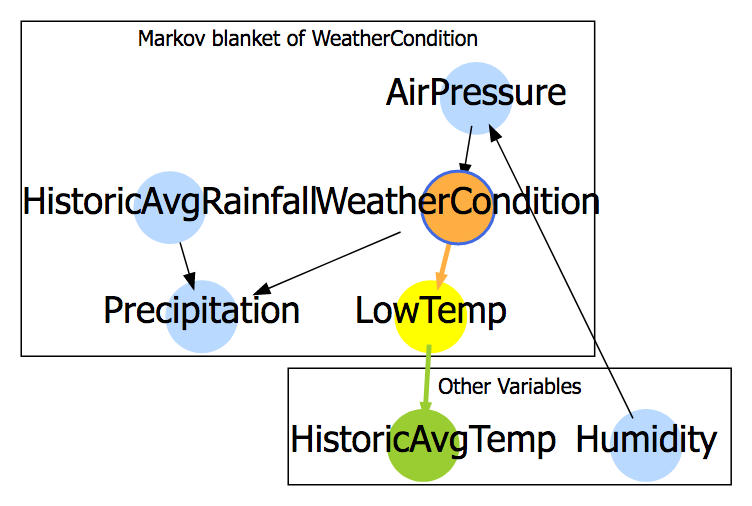
\includegraphics[width=1\textwidth]{CausalGraph1}
    \end{minipage}\hfill
    \begin{minipage}{0.5\textwidth}
        \centering
        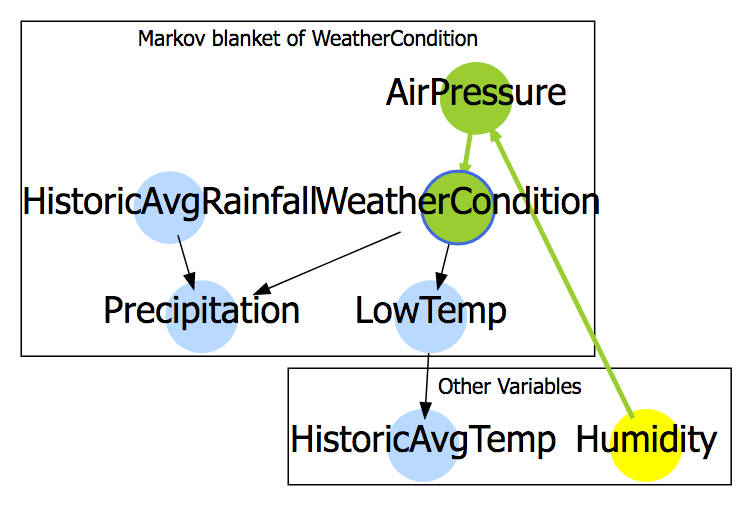
\includegraphics[width=1\textwidth]{CausalGraph2}
    \end{minipage}
    \caption{\textbf{Highlighting Information.} (A) The selected feature is highlighted yellow; direct causes are highlighted orange; direct effects are highlighted green. Low Temperature's Markov blanket consist of a direct cause, weather condition, and a direct effect, Historic Average Temperature. (B) The path to weather condition is highlighted green. Humidity affects weather condition though air pressure.}
    \label{fig:CausalGraphs}
\end{figure}

\subsection{Modifying the Causal Network}
The user can modify the graph to reflect their prior knowledge about the causal relationships between features. For example, the user can remove a feature that the user suspects or believe may not be relevant to the classification task. The feature is removed from the observed data and the causal graph will be rebuilt.

Moreover, the user can remove edges representing relationships that conflict with the user’s prior knowledge and also add new directed edges to represent relationships not captured in the graph. The system prevents the user from adding edges that introduces a cycle. Modifications to the graph may change the Markov blanket features of the target, and consequently, the graph will update to reflect the new information. Graph modifications can be undone and the graph will be reverted.

Initially, the possible graph edits are edge addition, edge removal, and feature removal. We observed during the pilot of the evaluation study that participants made many edges reversals. In order to reverse an edge, they first remove an edge $X \rightarrow Y$, let the graph update, and then add a new edge $Y \rightarrow X$. We added edge reversal as a fourth possible graph edit in order to condense a two-step edge reversal to one step.

\subsection{Markov blanket (MB) Consistency Score} \label{MBConsistencySubsection}
The Markov blanket consistency score is another metric used for measuring the consistency of the feature set to the prior knowledge. The MB consistency score measures the consistency of the feature set in relation to the causal relationships established. As described in subsection \ref{MarbovBlanket}, a node's Markov blanket variables cut it off from the influence of other variables in the network and are predictive of the node. To stay consistent with the idea that the Markov blanket is predictive, the consistency of the selected features to the target's Markov blanket is calculated. MB score is the fraction of the Markov features that are “covered” by a subset of the selected feature set. A Markov blanket feature is “covered” if a subset of the selected features form a connected path to the feature or is a selected feature. Let \(B\) be the set of Markov blanket features, the MB Score is expressed as

\begin{equation}
\label{eqn:MBConsistency}
MB Score = 
\sum_{f \in B}
    \begin{cases}
      1/|B| & \text{if f is covered}\\
      0 & \text{otherwise}
    \end{cases} 
\end{equation}

A Markov blanket feature is given the same score as a subset of features that form a connected path to the Markov blanket feature. The user may not want to use a Markov blanket feature for various reasons, such as the feature may be difficult or costly to measure. The user can consider replacing the Markov blanket feature with related features, and there are various ways the user can interact with the graph to find replacements. First, the user can highlight the feature's Markov blanket to identify features that directly influence it. For example, in figure \ref{fig:CausalGraphs}, low temperature is in the target's Markov blanket, and historic average temperature (highlighted in green) is a direct effect of low temperature. We can replace low temperature with historic average temperate in a feature set and low temperate would be covered. Second, the user can also highlight connected paths between a feature and target. For example in figure \ref{fig:CausalGraphs}, humidity has a path to weather conditions through air pressure. We can replace air pressure with humidity in a feature selection, and air pressure would still be covered. 

\section{Exploring Feature Space}
\begin{figure}[!htbp]
\centering
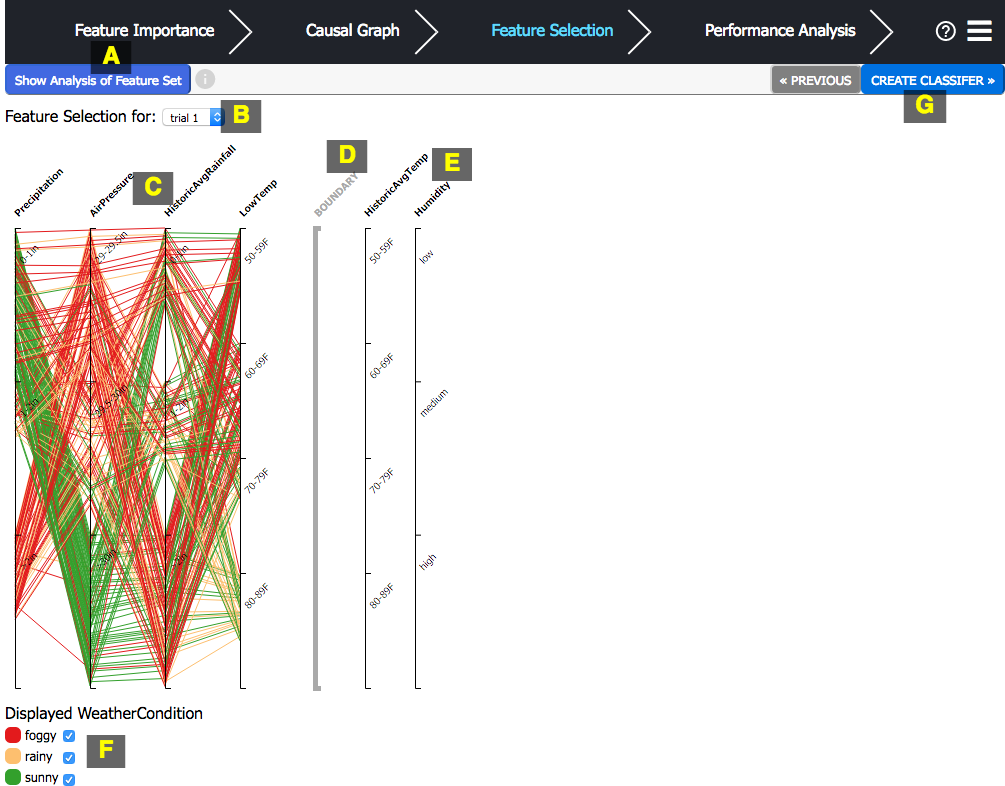
\includegraphics[width=1\textwidth]{LabeledFSInterface}
\caption{\textbf{Exploring Feature Sets Interface.} (A) Click ``Show Analysis of Feature Set" to switch to the analysis view. The analysis view is used to evaluate current feature selection against previously established prior knowledge. (B) The user can select to display the feature selection for previously trained models. (C) Features are represented as vertical axes. Features to the left of the BOUNDARY axis are in the selected feature set. Each line represents an example and intersects a feature axis at the feature value for that example. The line color corresponds to the target label of the example. (D) The BOUNDARY axis separates the selected features on its left from the not selected features on its right. (E) Lines representing examples do not extend beyond the BOUNDARY axis to the feature axes that are not selected. (F) The legend correlates color to target label. The user can also select which target labels to be displayed on the interface. } \label{fig:LabelFSInterface}
\end{figure}

After feature importance and causal relationships have been established, the user explores possible feature sets. We designed the feature selection interface to support interactive exploration of the feature space, to identify patterns in the dataset, and to evaluate the consistency of a feature set in relation to prior knowledge. Components are designed to communicate information about features. Prior knowledge is integrated to help the user filter features. The interactions are designed to support the efficient exploration of feature space and comparison of feature sets. 

The design of the feature selection interface and interactions also attempts to prevent overfitting. We enable the user are able to utilize their prior knowledge and the visual components for describing prior knowledge discussed in the later section to manual select predictive features and filter out not predictive features. As opposed to the common feature selection methods that limit the control of the user at selecting features, the user can easily add or remove features from the selected feature set based on information about feature importance and causality and help the system prevent overfitting.   

A feature is represented as a vertical axis, identified by the feature name at the top of the axis. A continuous feature axis ranges from the minimum to the maximum feature value. A discrete feature axis is equally partitioned into its feature values. The BOUNDARY axis separates the selected features on its left from the not selected features on its right as shown in figure \ref{fig:FSCorrelation}. 

The default feature set is the target's Markov blanket, which is consistent with the previously expressed information and has a Markov blanket consistency score of 1.0. A default model is created using the target's Markov blanket features and labeled as the trial 0 model. The user can compare the consistency of a feature set and performance of a model against the default model and should attempt to create a model that performs better. 

\subsection{Displaying Examples}
Examples are incorporated into the visual to identify patterns between feature values and target labels. Each example is represented by a line. The color of the line corresponds to the target label of the example. The line intersects a selected feature axis at the example's feature value and does not extend beyond the BOUNDARY axis to unselected feature axes. For continuous features, the line intersects the continuous axis at the feature value. For discrete features where a partition of the axis corresponds to a value, the line intersects the next available point in the value partition. Discrete feature values are a partition of the axes rather than a point to prevent many lines from converging at a specific value on the axis which may mislead the user on how many examples are represented by the line. Separating the examples with the same discrete feature value also helps better identify patterns and correlations between feature values. 

\subsection{Interactive Feature Selection}
The interface is designed to enable the user to interactively select features. Features can be added or removed from the selected feature set by dragging the feature axis to the left of the boundary or right of the boundary, respectively. Moreover, the boundary axis can also be dragged so that features to its left are selected and features to its right are not selected. The visualization enables users to interactively and quickly select a feature set and efficiently make elementary modifications to the feature selection. This helps the user efficiently explore and analyze different feature sets. The graph dynamically updates after a feature axis is repositioned. Other visual components and calculations that depend on the selected feature set also dynamically update. Features can be repositioned to help identify patterns or correlations. For example, figure \ref{fig:FSCorrelation} shows the correlation between feature values in the first axis, Air Pressure, and feature values in the second axis, Humidity. Examples with air pressure greater than 30in are likely to have a medium level of humidity. 

\begin{figure}[!htbp]
\centering
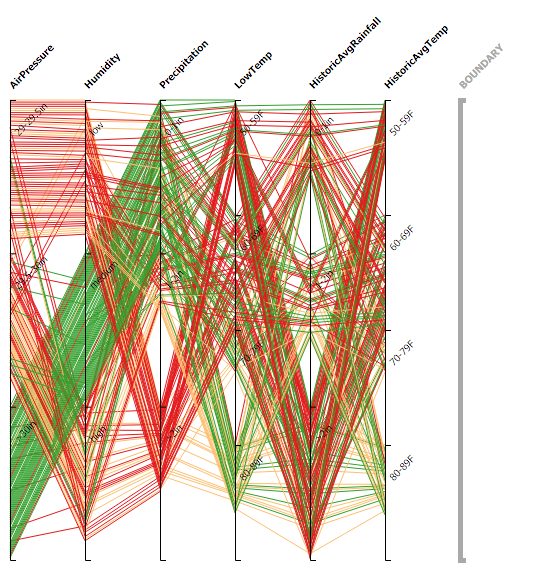
\includegraphics[width=0.65\textwidth]{FSCorrelation}
\caption{\textbf{Correlation Between Features.} Air pressure is correlated to humidity. Examples with air pressure greater than 30in is highly likely to have medium level of humidity, while examples with air pressure between 29-29.5in is more likely to have low level humidity} \label{fig:FSCorrelation}
\end{figure}

\subsection{Filtering Visual Information}
Filtering functionalities are implemented to allow the user to reduce the amount of visual information and better identify patterns. First, the user can select and deselect which target labels to display. When a target label is deselected, the graph dynamically updates the color of unselected examples to a light gray. Skewed datasets can be detected since the color of the dominating target label will dominate the graph. Another benefit of filtering is that the user can filter out dominating target labels and focus on the less frequent target labels. Moreover, filtering for a specific target label can help the user visually identify feature values that are related to that target label \ref{fig:FilterTargetLabel}.

\begin{figure}
    \centering
    \begin{minipage}{0.7\textwidth}
        \centering
        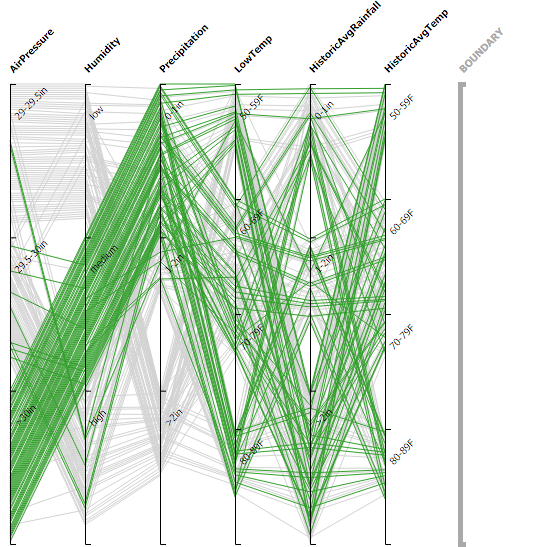
\includegraphics[width=.85\textwidth]{FilterTargetLabel}
    \end{minipage}\hfill
    \begin{minipage}{0.3\textwidth}
        \centering
        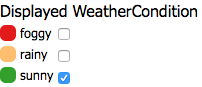
\includegraphics[width=1\textwidth]{FilterTargetLabelLegend}
    \end{minipage}
    \caption{\textbf{Filter Target Label}. User filtered for sunny examples/days. The visual shows that greater than 30 in air pressure, medium (30-60\%) humidity, and 0-1in precipitation are weather metrics that are correlated to tomorrow's sunny weather condition.}
    \label{fig:FilterTargetLabel}
\end{figure}

In addition, the user can filter for feature values by highlighting a range in the feature axis. Feature ranges can be highlighted for multiple feature axes. The entire feature range is used by default for features without a specified filter range. Each time a filter is updated, the graph dynamically grays the lines representing examples whose feature values are not in all of the specified feature ranges. Filtering for feature value can help the user visually identify patterns. For example, in figure \ref{fig:FilterTargetLabel}, after the user had filtered out rainy and foggy examples, the graph reveals that most of the sunny examples have precipitation between 0 and 1 inch the previous day. Filtering by feature values can also help identify which sets of feature values may distinguish a target label as shown in figure \ref{fig:FilterValues}.

\begin{figure}[!htbp]
    \centering
    \begin{minipage}{0.7\textwidth}
        \centering
        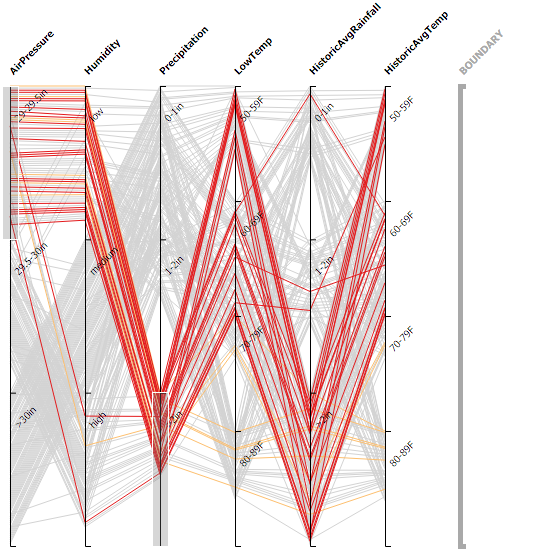
\includegraphics[width=.85\textwidth]{FilterValues}
    \end{minipage}\hfill
    \begin{minipage}{0.3\textwidth}
        \centering
        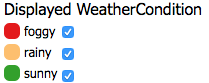
\includegraphics[width=1\textwidth]{FilterValuesLegend}
    \end{minipage}
    \caption{\textbf{Filter Feature Values}. User filters for examples/days with air pressure between 29.0 and 29.5in and precipitation of greater than 2 in. The interface reveals that examples with both these metrics are more likely to have foggy weather conditions.}
    \label{fig:FilterValues}
\end{figure}

\begin{figure}[!htbp]
\centering
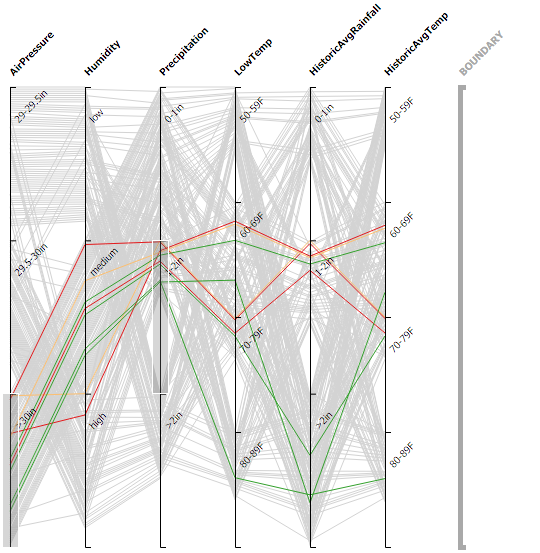
\includegraphics[width=0.65\textwidth]{FilterValuesSparse}
\caption{\textbf{Uncorrelated Feature Values}. User filtered for examples/days with air pressure greater than 30.0in and precipitation between 1 to 2in. All possible target labels are represented in the few examples that are unfiltered, which reveals that these two feature values are most likely uncorrelated or rarely occur together.} \label{fig:FilterValuesSparse}
\end{figure}

\subsection{Metrics for Analyzing Feature Set}
\begin{figure}[!htbp]
\centering
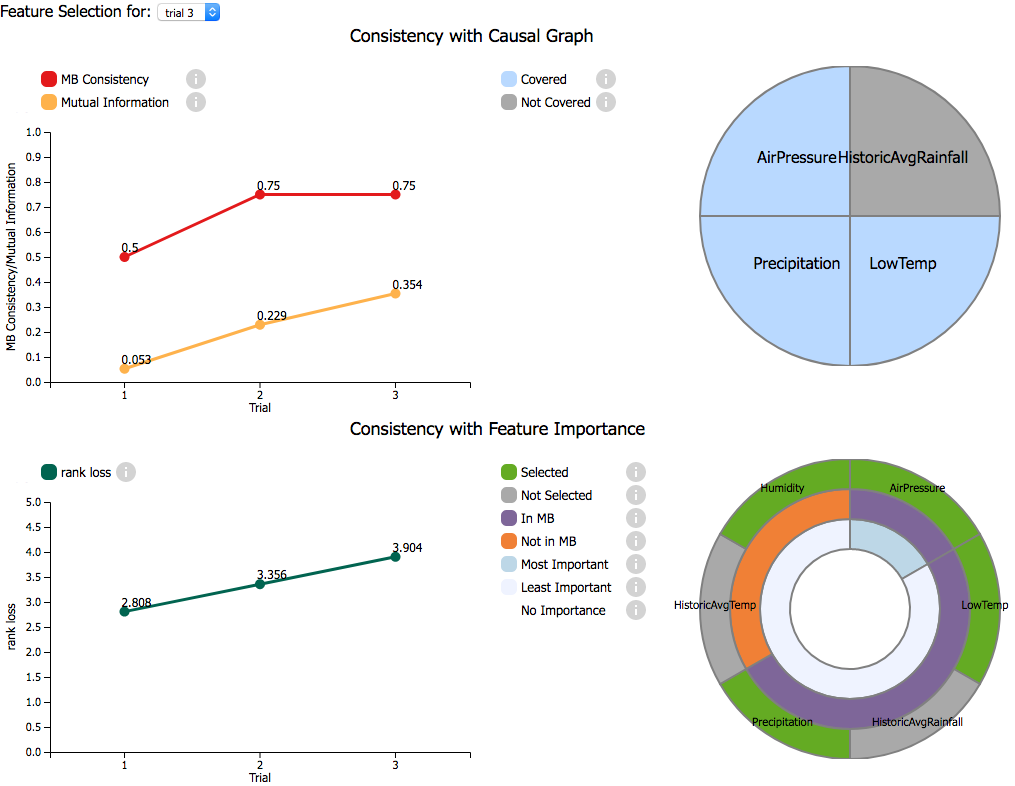
\includegraphics[width=1\textwidth]{FeatureAnalysisInterface}
\caption{\textbf{Feature Selection Analysis Interface.} At the feature selection step, user can switch to the analysis view to assess metrics and graphs that help determine whether the current feature set is a good choice and whether it is consistent to the user's prior knowledge.} \label{fig:FeatureAnalysisInterface}
\end{figure}

Metrics are calculated to describe how consistent a feature set is to feature importance and causalities expressed in previous steps. Scores are dynamically calculated and updated each time the feature selection changes. The three metrics calculated are Markov blanket (MB) consistency score, mutual information (MI) score, and rank loss.

\subsubsection{Markov Blanket Consistency Score and Coverage Pie Chart}
The MB score describes the feature set consistency in relation to causalities expressed in the Bayesian network build in the previous step. Refer to section \ref{MBConsistencySubsection} and equation \ref{eqn:MBConsistency} for the MB score calculation. The MB score has a range of [0.0, 1.0], where 1.0 corresponds to all features being covered and 0.0 corresponds to none of the features being covered. The default feature selection with the Markov blanket features has a score of 1.0. The feature set that maximizes the Markov blanket score is not unique. The user can attempt to maximize the score to stay consistent with established prior knowledge.

In complementary to the score, a pie chart visually shows which Markov blanket features are covered as shown in figure \ref{fig:CoverageChart}. The pie chart is equally divided into slices that correspond to the set of Markov blanket features. Covered features are highlighted blue, while uncovered features are highlighted gray. The fraction of blue on the chart corresponds MB score that reports the fraction of covered features. Since the score and chart are dependent on the previously provided information, modification to the causal graph will cause the pie chart to update with the new Markov blanket features and the score to be recalculated.

\begin{figure}[!htbp]
    \centering
    \begin{minipage}{0.5\textwidth}
        \centering
        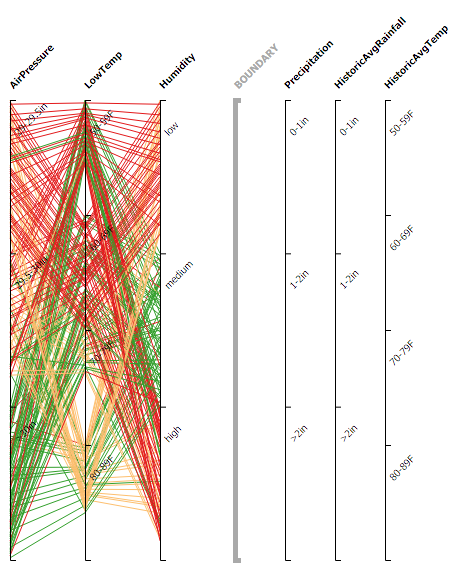
\includegraphics[width=1\textwidth]{SelectedFeaturesCoverage}
    \end{minipage}\hfill
    \begin{minipage}{0.5\textwidth}
        \centering
        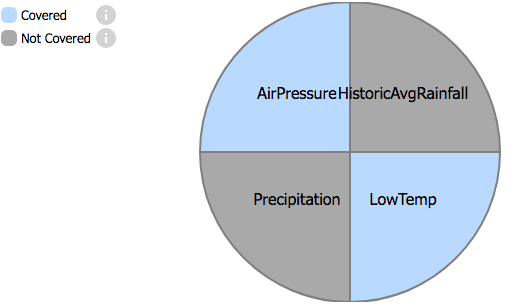
\includegraphics[width=1\textwidth]{CoverageChart}
    \end{minipage}
    \caption{\textbf{Markov Blanket Feature Coverage Chart.} The chart is composed of the four features that make up the target's Markov blanket. Air pressure and low temperature are in the selected set and are covered, while precipitation and historic average rainfall are not in the selected set and are not covered. } \label{fig:CoverageChart}
\end{figure}

\subsection{Mutual Information (MI) Score}
The MI score is computed using Mutual Information Maximization (MIM) scoring criterion \ref{eqn:MIM}, which can use as a criterion in filter-based feature selection methods. Mutual information is a measure of the amount of information that one random variable has about another random variable. The mutual information between two independent features is 0. The MIM score expresses the sum of the information shared between the selected features and the target in terms of entropy. The MI score can also support users at filtering features. For example, if the addition of a feature increases the MI score significant, then the feature has information about the target. On the flip side, if the score does not increase by much, then the feature does not have much information about the target. However, MIM does not account for the redundant information a feature has about the target that may already be accounted for by another feature in the selection. 
A mutual information score is incorporated in the analysis because information measure based metrics are commonly used to filter for features, and therefore can be used for assessing the feature selection. The MI score is calculated as an additional predictor of whether the selected feature set will result in a high performing model. MIM function can be replaced by other mutual information functions or more mutual information scores can be incorporated into the interface. 

\subsection{Rank Loss and Feature Importance Consistency Chart}
\begin{figure}[!htbp]
\centering
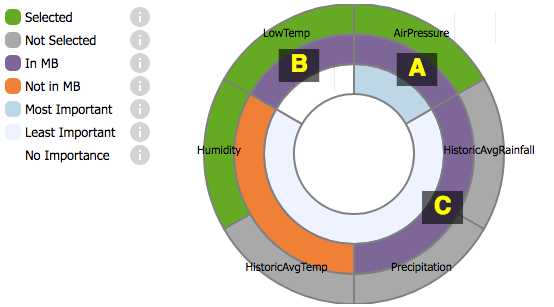
\includegraphics[width=0.75\textwidth]{SunburstChartLabeled}
\caption{\textbf{Feature Importance Consistency Chart.} (A) Air Pressure is the most important feature and is part of the feature selection. (B) However, Low Temp, the least important feature is also apart of the feature selection. (C) Half of the Markov blanket features are not included in the feature selection.} \label{fig:SunburstChart}
\end{figure}
Rank loss \ref{eqn:rankloss} expresses the consistency the feature set to the expressed feature importance. The minimum value of rank loss is 0. A feature selection that is consistent with feature importance minimizes rank loss. 

A complementary chart is designed to visually express the consistency of the feature selection to the feature importance information. The chart is a sunburst or multilevel pie chart used to encompass various levels of information. The outermost pie is equally divided into all the features. The second pie shows whether the adjacent feature in the outer circle is in the target's Markov blanket or not. Markov blanket features are filled in purple and non-Markov blanket features in orange. Lastly, innermost pie describes the importance of the adjacent feature - the color of the slice corresponds to the color of the circle the feature was grouped in during the feature importance step. 
In the outer circle, the features that are filled in green are part of the feature selection while the features filled in gray are not. By organizing the information in a multilevel fashion, the user can see if the more important features are included in the feature selection and also if Markov blanket features are relatively important.

\subsection{Progress Graphs}
\begin{figure}[!htbp]
    \centering
    \begin{minipage}{0.5\textwidth}
        \centering
        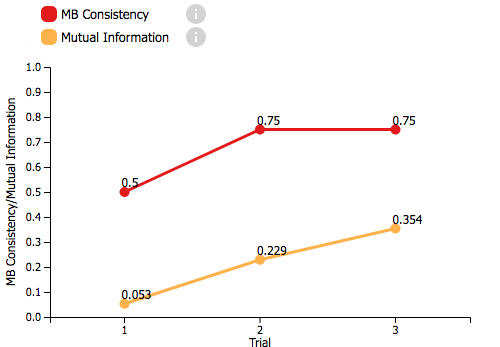
\includegraphics[width=1\textwidth]{MIGraph}
    \end{minipage}\hfill
    \begin{minipage}{0.5\textwidth}
        \centering
        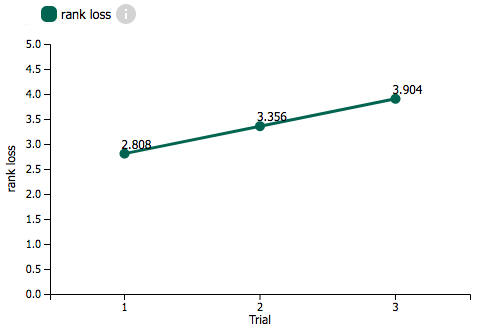
\includegraphics[width=1\textwidth]{RankLossGraph}
    \end{minipage}
    \caption{\textbf{Progress Graphs.} Metrics are used to assess whether the feature set may produce a high performing model and how consistent the feature set is to previously provided information. Metrics are calculated for each model and plotted to show the progress in model construction. MB consistency scores of the feature sets have increased since the first iteration, so more Markov features are covered in the later iterations. MI score has also increased, so the amount of shared information between selected features and target has increased. } \label{fig:ProgressGraph}
\end{figure}
The system enables the user to iteratively construct models. The progress of the models' metrics is tracked. The MB and MI scores are displayed in one graph and the rank loss score is displayed in a separate graph because maximizing the MB and MI scores corresponds to an increase in consistency while minimizing the rank loss score corresponds to an increase in consistency. Initially, the graphs only display the metrics for the first trial. The scores for the current feature selection dynamically update when the feature set updates. 

The system is designed for the iterative model building process. A model is built with the current feature selection. The user can continue to build models with different feature sets. A model is constructed at each iteration, which is labeled as a trial in the system. The information pertaining to previous trials, such as selected features, metrics, and model performance, is retained for the purposes of comparing and contrasting the models. The metrics for analyzing feature sets are displayed as a line graph to display the progress of the model creation process and also to compare the metrics of the different trials.  

\subsection { Classification Algorithm }
The system builds a model from the user selected features - the features on the left of the BOUNDARY axis. A basic classification algorithm is used to create the model. For the evaluation study, we use the k-nearest neighbors algorithm (kNN) for classification and set the number of nearest neighbors $k$ to use as 3. The kNN algorithm assigns an example to the target label that is most common among its $k$ nearest neighbors. The interactive feature selection system is designed to be model agnostic. In theory, the user will be able to specify the classification algorithm and its input parameters. The feature for allowing the user to pick the classifier and its parameters directly from the user interface has not been implemented.

Moreover, we perform stratified $k$ fold cross validation to access the accuracy and performance of the resulting classifier. The original dataset is randomly partitioned into $k$ equal sized subsets where the fractions of target labels equal that of the original data set. Of the $k$ subset, a single set is retained for testing the resulting classifier; the remaining $k-1$ sets are used as training data to create the classifier. The cross-validation process is repeated $k$ times. Each of the subsets is used once as testing data. Lastly, the $k$ results such as test accuracy is averaged to produce the overall test accuracy.

\subsection{Performance Analysis} \label{PASection}
The system incorporates performance analysis to assess the model. The user is automatically taken to the performance analysis interface after a model is built. Accuracy, the percentage of the examples whose target labels are correctly predicted, is a commonly used metric to assess a model's performance and is used at this step. 

Another component of the interface is the confusion matrix, which is a commonly used table for reporting classification results. The rows of the matrix correspond to the actual labels and the columns correspond to the model's predicted labels of the example. The matrix communicates how many examples of a label are predicted as the other target labels. A high performing model will have a high concentration of examples along the diagonal - as those cells correspond to how many examples of a label are correctly predicted as that label. However, because the dataset can be skewed towards a certain target label, the magnitude of the numbers along the diagonal may bias the viewer's assessment of the model's performance. To provide more information, the cells of the confusion matrix are colored using an orange color scale. The scale mapped to the accuracy range 0.0 to 1.0, where the lightest orange correlates to 0.0 and the darkest orange correlates to 1.0. The color represented the fraction of examples of a target label that are predicted as the target label corresponding to the column. A high performing model that correctly predicts examples has the darkest orange along the diagonal and light orange everywhere else. 

\begin{figure}[!htbp]
\centering
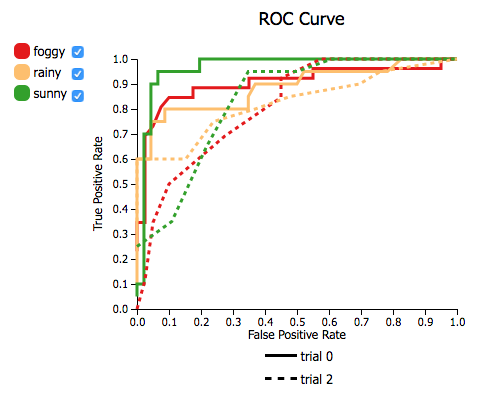
\includegraphics[width=0.75\textwidth]{ROCmultiple}
\caption{\textbf{ROC Curves.} The ROC curves for trial 0 and trial 3 models are plotted as solid and dotted lines respectively. The user can select to display the curves of certain target labels. A greater area under the ROC curve represents higher performance. By overlaying ROC curves of two models, we can see which curve has a greater area under the curve and determine which model performs better.} \label{fig:ROCmultiple}
\end{figure}

Receiver operating characteristic (ROC) curves are used for visual performance analysis. The ROC curve is created by plotting the true positive rate against the false positive rate at various probability thresholds. The model often provides confidence scores for their predictions - for example, the model may be 67\% certain that this example's weather condition is sunny. The probability threshold, a parameter often set by the user, is how certain the model has to be before it can make its prediction. 
For classification problems where there are three or more possible labels, an ROC curve is plotted for each of the labels. Each curve plots the rate the model correctly predicts examples of that label against the rate the model incorrectly predicts the examples as any of the other labels as shown in figure \ref{fig:ROCmultiple}. The area under the curve (AUC) is an indicator or the model's performance. A greater area under the curve represents higher performance. 

\begin{figure}[!htbp]
\centering
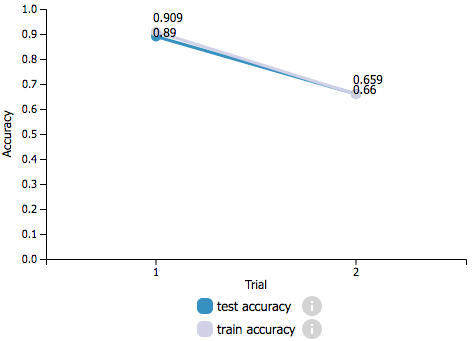
\includegraphics[width=0.75\textwidth]{accuracy}
\caption{\textbf{Accuracy Graph.} The training and testing accuracy of each iteration are plotted to show the progress and to compare models. Training accuracy is the fraction of examples in the training set that the model correctly predicted; testing accuracy is the fraction of unseen examples that the model correctly predicted. In this figure, the first trial has greater training and testing accuracy than the second trial. } \label{fig:accuracy}
\end{figure}

\subsection{Comparing Models}
\begin{figure}[!htbp]
\centering
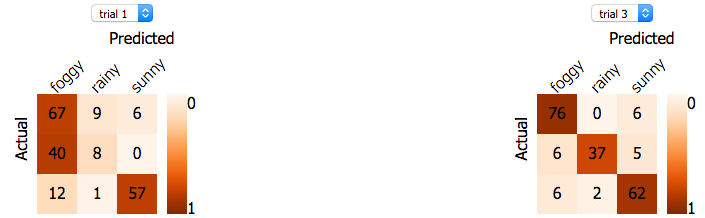
\includegraphics[width=1\textwidth]{ConfusionMatrixCompare}
\caption{\textbf{Comparing Model Performances.} We compare the third model with an accuracy of 0.87 against the first model with an accuracy of 0.66. The third model's confusion matrix has darker orange along the diagonal, which indicates it has a higher percentage of correctly predicted examples for each of the target labels. On the other hand, the first model's confusion matrix shows that its confusing many rainy examples for foggy examples. } \label{fig:ConfusionMatrixCompare}
\end{figure}

\begin{figure}[!htbp]
\centering
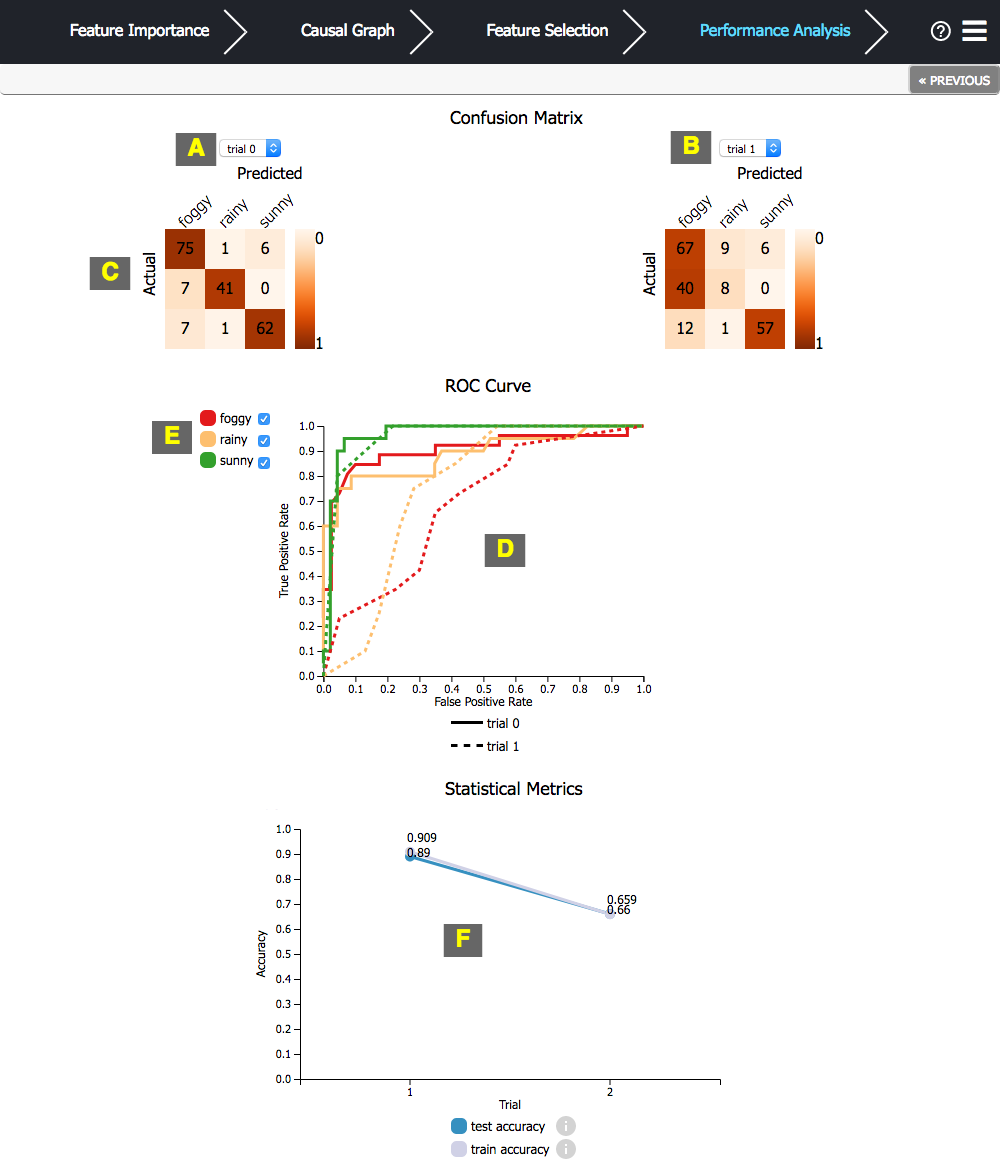
\includegraphics[width=1\textwidth]{compareclassifierspageview}
\caption{\textbf{Comparing Model Performances.} We compare the third model with an accuracy of 0.87 against the first model with an accuracy of 0.66. The third model's confusion matrix has darker orange along the diagonal, which indicates it has a higher percentage of correctly predicted examples for each of the target labels. On the other hand, the first model's confusion matrix shows that its confusing many rainy examples for foggy examples. } \label{fig:PerformanceAnalysisPage}
\end{figure}

The performance analysis step is designed for iterative model creation. Training and testing accuracies are displayed in a line graph to show the progress of the model creation process. The graph can also be used to compare the accuracy of different models. Moreover, two confusion matrices are shown side by side for the purpose of comparison. By default, when a new model is created, the left confusion matrix is updated to display performance of the newest created model and the right matrix is updated to display the previous model created. The user can choose which trial's confusion matrix to display and which models to compare by selecting the trial to display using the selection element above the confusion matrix, as shown in figure  {fig:PerformanceAnalysisPage}.

The user can also compare model performances using the ROC curve. The user can select which two trials' ROC curves to display. One trial's curves will be in solid while the other's curves will be dotted as shown in figure \ref{fig:ROCmultiple}. Since the area under the curve is an indicator of model performance, ROC curves are well fit for visually comparing performance. By overlaying curves from different models, we can see which model produces curves with larger areas. Moreover, the user can also select which target label's curve they want to be displayed.  

Moreover, the system retains information about previous trials to show which feature sets were already tried. To correlate the performance of the model with the feature set used to create the model, the user set the corresponding trial to display at the feature selection step. Then, the interface for the feature selection step and the graph for assessing the feature set updates to reflect the feature set used for the selected trial. In addition to selecting previously selected feature sets for comparison, the user can also select high performing iterations and make changes to that feature set in attempt to create a higher performing classifier. This function is used by participants during the user study to improve on previously selected feature sets. The interface and interactions are designed to enable the user to compare and contrast models and visually keep track of their model creation progress. They help with the iterative nature of the classification progress by showing the progress of the iterations, retaining information about the previous iterations, and enabling the user to access feature sets from previous trials and then modified the original feature set. 


\cleardoublepage
\chapter{Evaluation}
%importance of evaluation
Evaluation is important to assess the ability and design of visuals in achieving their purpose. We conducted a user study to evaluate the system and its effectiveness at facilitating collaborative feature selection. In this chapter, we first outline the purpose and focuses of the evaluation and then explain its procedure. Later in this chapter, we describe the series of tasks that make up the study, explain how the tasks evaluate the system and explain the results of the tasks.

\section{ Objectives of the Evaluation Study }
The three main foci of the evaluation study aimed to understand the user interface's effectiveness at facilitating collaborative feature selection and the interpretability of the visualizations. Qualitative and quantitative evaluation methods are utilized to answer specific research questions.

\subsection{Research Questions}
Specific research questions extend from the main foci of the evaluation study. The research questions for the study are organized into three categories - effectiveness of the system, interpretability of the visualizations, and the exploration of feature space. The research questions are listed below.

Effectiveness measures the ability of the user interface to help the user accomplish their task.
\begin{itemize}
\item{Is the design of the application intuitive to the user?}
\item{Does the user build a classifier with high performance?}
\item{Does the built classifier reflect causal aspects accurately?}
\item{Does the built classifier reflect feature importance accurately?}
\end{itemize}

Interpretability measures the ability of the visuals to correctly and efficiently communicate information.
\begin{itemize}
\item{Are the visuals produced by the application easy to read?}
\item{Are the visuals correctly analyzed by the user?}
\item{Can the user explain/interpret the feature set used to build the classifier? }
\item{Can the user explain/interpret why a certain feature set may create a higher performing classifier than another feature set?}
\item{Does each piece contribute to the overall interpretability? I.e. if the causal graph is removed, is it more difficult to explain the classifier’s performance?}
\end{itemize}

Exploration of feature space measures the ability of the application to help the user make feature selections and identify a subspace of predictive feature sets.
\begin{itemize}
\item{Does the design of the application aid in feature exploration?}
\item{How quickly can a user select the most relevant features?}
\item{How quickly can a user filter out the most irrelevant features?}
\item{How quickly can the user choose between features that directly influence the label versus indirectly influence the label?}
\end{itemize}

\section { Methodology }
\subsection { Version B }
For the evaluation study, we create a separate application that does not incorporate prior knowledge about feature importance or causal relationships. The original application will be referred to as version A and the participants using version A are in group A, while the limited application will be referred to as version B and those participants are in group B.

The only two steps in version B are feature selection and performance analysis as shown in figures \ref{fig:LabelFSInterface} and \ref{fig:PerformanceAnalysisPage}. Group B's behavior and responses are compared against group A's to determine the effects that integrating prior knowledge has on feature selections, the number of trials performed during feature selection, the total time for the feature selection process, and other behaviors.

\subsection{ Participants }
Participants are recruited from the undergraduate and graduate students at Case Western Reserve University. First, they are provided with a high-level overview of the study and consent to participating in the study and having unidentifiable data collected. Participants then answer a questionnaire about their major and knowledge of machine learning and classification, which is used to divided them equally into group A and group B. When assigning participants to a group, we match two participants with similar characteristics and divide them between the two groups. The characteristics we use to match participants are major, age, and experience in machine learning. Participants in group A and B are further specified based on whether they majored in computer science (CS) or not. The number of participants in and information about group A and B are presented in table \ref{ParticipantInfo}.

\begin{table}[]
\centering
\begin{tabular}{lcc}
\hline
Participants &  \multicolumn{1}{l}{Version A} &  \multicolumn{1}{l}{Version B} \\ \hline
CS           & 10        & 5        \\
Other       & 5         & 5         \\ \hline
\textbf{Total}        & \textbf{15}        & \textbf{10}        \\ \hline
\end{tabular}
\caption{Participants are grouped by which system they are evaluating and whether they major in CS or not. The number of participants in each group is reported. }
\label{ParticipantInfo}
\end{table}

\subsection {Design of the Evaluation}
The system is designed for users with basic knowledge and understanding of machine learning and classification. In the introductory material (figures \ref{fig:IntroMaterials1}, \ref{fig:IntroMaterials2}), participants are given brief explanations about classification and feature selection, an example of a use case for the system, and necessary terminologies - such as accuracy, target label, etc. They are trained through a series of short introductory videos that explain the feature selection workflow, the system functionalities, and the interface visualizations. The tutorial features a weather classification problem that is classifying tomorrow's weather conditions as either sunny, rainy, or foggy based on today's weather metrics. After processing the introductory materials, participants interact with the system that shows the demonstration dataset. After they are familiarized with the system, they proceed to the user study.

\begin{figure}
    \centering
    \begin{minipage}{0.5\textwidth}
        \centering
        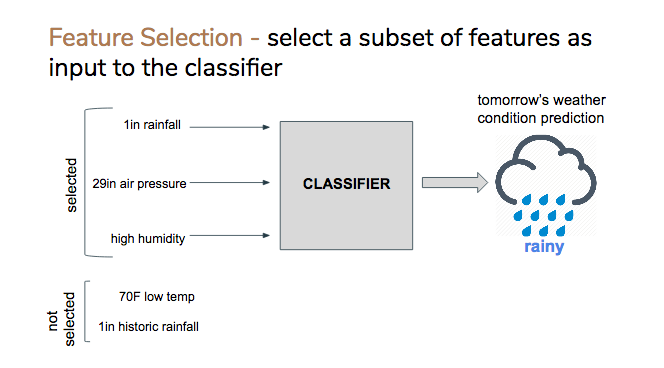
\includegraphics[width=.85\textwidth]{intromaterial1}
    \end{minipage}\hfill
    \begin{minipage}{0.5\textwidth}
        \centering
        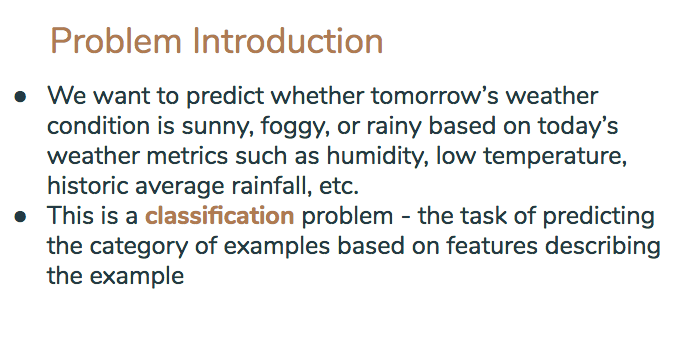
\includegraphics[width=1\textwidth]{intromaterial2}
    \end{minipage}
    \caption{\textbf{Introductory Material}. (Left) The slide introducing the demonstration classification example - predicting tomorrow's weather condition using today's weather condition. (Left) The slide explaining feature selection using the demonstration example. }
    \label{fig:IntroMaterials1}
\end{figure}

\begin{figure}
    \centering
    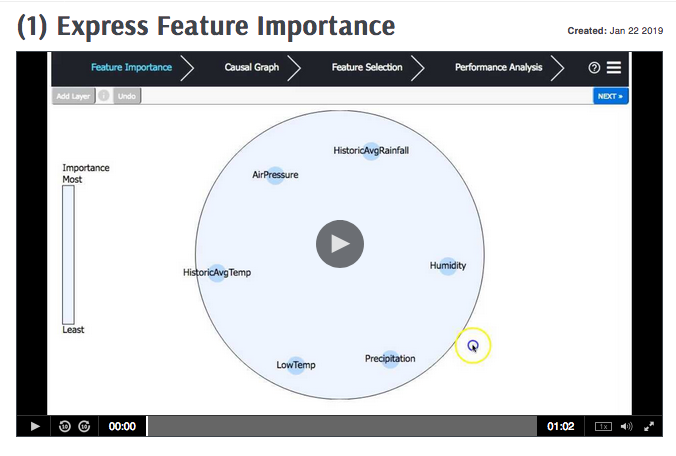
\includegraphics[width=.85\textwidth]{intromaterial3}
    \caption{\textbf{Demonstration Video}. Participants watched a series of videos that explained the user interface and system functionalities. The first video the participants watched was on expressing feature importance. }
    \label{fig:IntroMaterials2}
\end{figure}

\subsection { Gathering User Interaction Data }
During the evaluation process, a tracking mechanism traces the participant's actions such as interactions with the graph, edits to the graph, moving features to a different circle, etc. Using the tracking mechanism, we can measure the time spent on each task, record the interactions performed to accomplish each task, and the correctness of their answer. The events are tracked and logged by keen \cite{keen}, an application for tracking and analyzing user interactions. Events are analyzed to extract quantitative results about the effectiveness and usability of the system.

Some tasks require the participants to interact with the interface, such as ``You think that today's humidity is important for predicting tomorrow's weather. Express this knowledge using the system". In addition, some tasks require written responses to understand if the participants correctly interpret the visualizations - such as ``What are the Markov blanket features of the target variable".

\section { Background Information }
The participants were presented with a specific scenario. The participants were told that they are developing a classifier for predicting student's letter grades (A, B, C, or F) based on information about the student such as whether they work a part-time job or participate in extracurricular. They were instructed to first read the descriptions of each feature which are presented in the sidebar of the application, as shown in figure \ref{fig:featuredescriptions}. Feature and the target variable descriptions presented to the participants are shown in table \ref{featuredescription}.

\begin{figure}
    \centering
    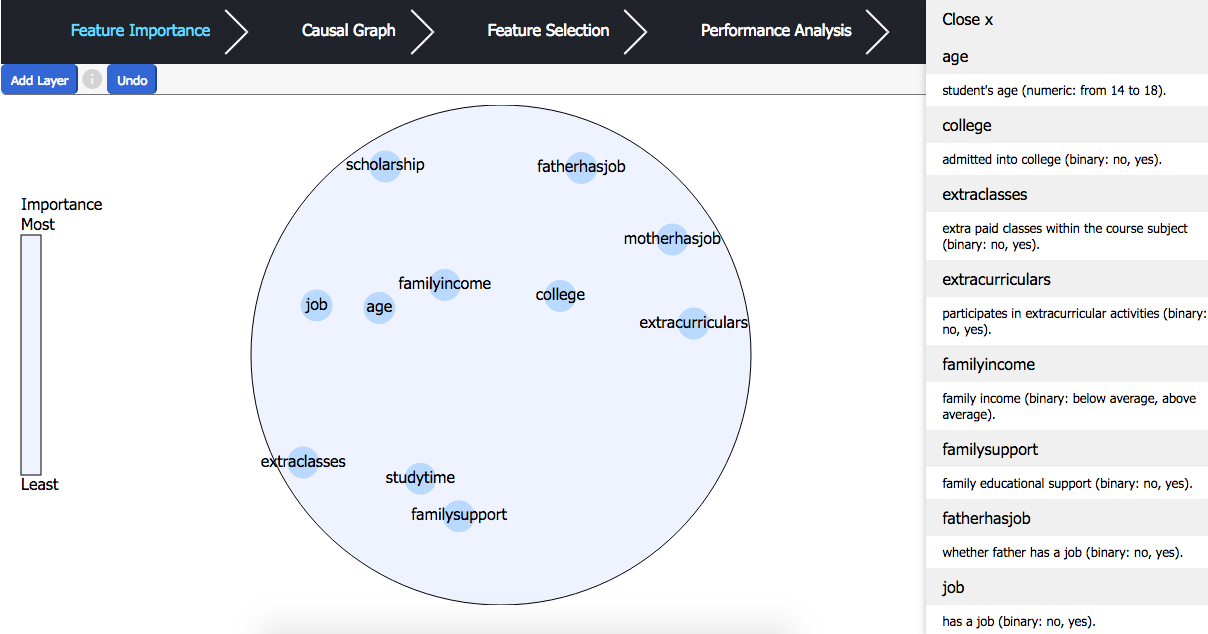
\includegraphics[width=.8\textwidth]{featuredescriptions}
    \caption{\textbf{ Feature Descriptions }. Participants were instructed to read feature descriptions presented on the sidebar of the interface. }
    \label{fig:featuredescriptions}
\end{figure}

\begin{table}[]
\centering
\begin{tabular}{lll}
\hline
Variables & Description & Values \\ \hline
motherhasjob & whether mother has a job & no, yes \\
extracurriculars& participates in extracurriculars & no, yes \\
job & has a job & no, yes \\
studytime & weekly study time & $>$2hr, 2-5hr, 5-10hr, $<$10hr \\
age & student's age & 14 to 18 \\
fatherhasjob & whether father has a job & no, yes \\
familyincome & family income & below avg, above avg \\
extraclasses & take extra classes & no, yes \\
familysupport & family educational support & no, yes \\
college & admitted into college & no, yes \\
scholarship & has scholarship for college & no, yes \\
grade & student letter grade & A B C F \\ \hline
\end{tabular}
\caption{Description of the features presented to the participants before they started the tasks.}
\label{featuredescription}
\end{table}

\subsection { Data Generation }
The dataset used for the evaluation study was generated from a Bayesian network created in pgmpy \cite{pgmpy}, a python library for working with probabilistic graphical models. First, the edges to and from variables representing features are defined. Then, the conditional probability distribution for each variable is defined. The actual Bayesian network that generated the data is shown in figure \ref{fig:actualBN}. 

After the Bayesian network is created, we generate samples from joint distribution of the Bayesian network. 500 examples are sampled from the Bayesian network to create the evaluation data set. 

\begin{figure}
    \centering
    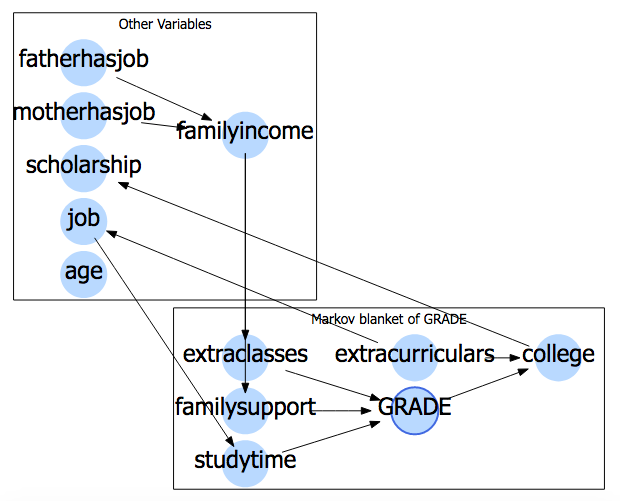
\includegraphics[width=.8\textwidth]{actualBN}
    \caption{\textbf{ Actual Bayesian Network of Evaluation Data set.}}
    \label{fig:actualBN}
\end{figure}

\subsection{ Evaluation Study Classification }
The interactive feature selection system is designed to be model agnostic. In theory, the user will be able to specify the classification algorithm and its parameters. For the evaluation study, we use the k-nearest neighbors algorithm (kNN) for classification and set the number of nearest neighbors $k$ to use as 3. kNN assigns an example to the target label that is most common among its $k$ nearest neighbors.

Moreover, we perform stratified 5 fold cross validation. The original dataset is randomly partitioned into 5 equal sized subsets where the fractions of target labels equal that of the original data set. Of the 5 subset, a single set is retained for testing the resulting classifier; the remaining 4 sets are used as training data to create the classifier. The cross-validation process is repeated 5 times. Each of the subsets is used once as testing data. Lastly, the 5 results such as test accuracy is averaged to produce the overall test accuracy.

\section { Evaluation Study }
We describe the background information presented to the participants and the instructions for each of the evaluation tasks.

The participants were told they will complete a series of tasks that will guide them to select features that will predict student grades. The tasks evaluate the feature selection process and the results will help answer the research questions. The tasks will be described later in this section. The tasks were presented one after the other and were to be completed consecutively. If the participant was unable to answer the question using the system or did not want to perform a task, they could proceed onto the next task without completing the task.

\subsection { Task 1: Express Feature Importance }
After the participants finished reading the feature descriptions, they proceeded to the first task. Task 1 evaluates the express feature importance step. 

Participants were informed that whether a student takes extra classes may be important for predicting their grade and that whether a student is admitted to college may be important but not as important as whether they take extra classes. 

Participants were instructed to express the importance of these features as well as their own ideas about which features are important for predicting student grades. The placement and grouping of features were logged and compared against the information provided in the task. This task was only completed by group A. 

Task 1 assesses the effectiveness of the interface and its interactions at helping the user express feature importance. Task 1 also evaluates the intuitiveness of the visualization and interactions. 

\begin{figure}
    \centering
    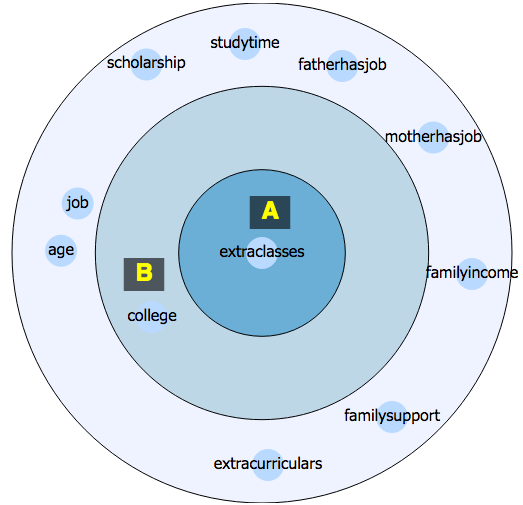
\includegraphics[width=.65\textwidth]{task1}
    \caption{\textbf{ Express Feature Importance Task }. The correct execution of the task places (A) extraclasses, the most important feature, in the innermost circle and (B) college in the adjacent circle. }
    \label{fig:Task1}
\end{figure}

\subsection { Task 2: Edit and Build Causal Graph }
The participants were then instructed to proceed to the next step which was expressing causal relationships. The GES algorithm outputted a possible causal network and the system presented the network to the participant. 

The participants were asked to utilize the functionalities of the interface to edit the causal graph. They were asked to express that participating in extracurricular is a cause of having a part-time job and having family support is a cause of participating in extracurricular. Moreover, if there are relationships that did not make sense or seems backward, the participant could remove or reverse the edge. The participant could also add edges to represent relationships. A possible causal network after the participants completed the task is presented in figure \ref{fig:Task2}. This task was only completed by group A. 

Task 2 is design to test the effectiveness of the interface and interactions at helping the user express causal relationships and build a causal network. 

\begin{figure}
    \centering
    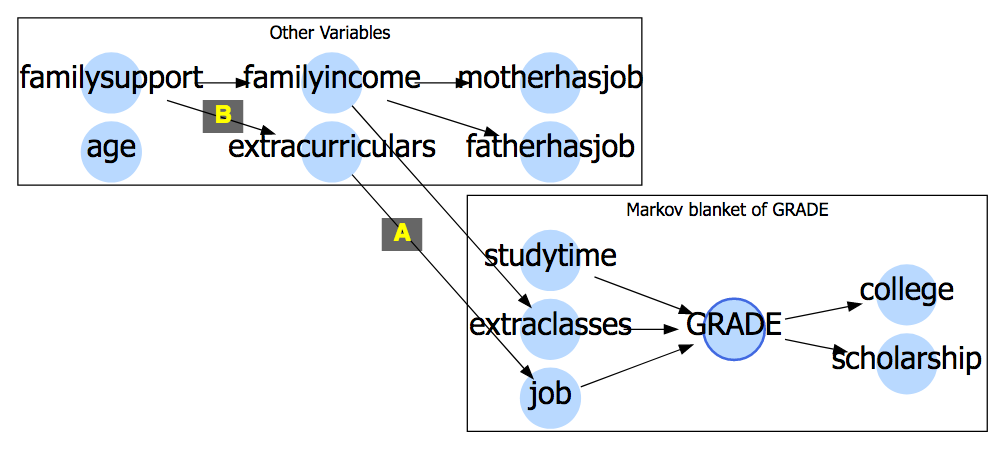
\includegraphics[width=.85\textwidth]{task2-2}
    \caption{\textbf{ Build Causal Graph Task }. A possible causal network of the dataset after the participant edit the graph to show (A) participating in extracurriculars as a cause of having a job and (B) having family support as a cause of participating in extracurriculars. The indirect causes of student grades are family income, family support, and extracurriculars. There are no indirect effects of student grades.}
    \label{fig:Task2}
\end{figure}

\subsection { Task 3: Interpret Causal Graph }
Task 3 was to be completed at the build causal network step. Participants were asked to identify indirect causes and effects of grade by reading and interacting with the graph. In figure \ref{fig:Task2}, the indirect causes of student grades are family income, family support, and extracurriculars and there are no indirect effects of student grades. This task is only completed by group A. 

Task 3 is design to evaluate the interpretability and readability of the causal graph.  The purpose of task 3 is to evaluate whether the built-in interactions such as clicking to highlight feature nodes help the user interpret the graph.

Furthermore, although group B did not complete this task or was presented with a causal network, they were asked to identify features that are causes or effects of student grades. We used their responses to access whether how causality helps participants select features; for example, whether participants are more likely to select features they thought were causes or effects of the target variable. 

\subsection { Task 4: Interpret Feature Selection Interface }
After the causal graph was built, the participants proceeded to the feature selection interface. The participants were given various questions that can be answered by reading the feature selection graph as shown in figure \ref{fig:LabelFSInterface}.

First, participants were asked to correlate a set of feature values - has scholarship and participates in extracurricular - to student grades.

Second, participants were asked to identify features that distinguish or separate A from F students and those that distinguish B and C students.

This task evaluates whether participants were able to correctly interpret the feature selection visual. Task 4 assesses the interpretability of the feature selection interface. This task is completed by both groups A and B. 

\subsection { Task 5: Analyze Feature Set Metrics }
Task 5 was to be completed using the feature analysis view that is part of the feature selection interface. Participants were directed to select and analyze a set of features that are not the set of Markov blanket features. The participants were asked to identify whether Markov blanket features are covered and whether important features were in the feature selection using the feature selection interface. They were also asked if and how the interface helped them arrived at their answers. The responses are used to assess whether the graphs and feature set metrics are being used and correctly interpreted. 

Lastly, the participants were asked to compare the feature set metrics of the current feature selection against trial 0`s, which was the set of target Markov blanket features. The responses are used to assess whether the graphs help participants determine the consistency of the current feature selection to previously expressed information. This question also evaluates the usability of the comparison function of the feature selection interface. 

The purpose of the task is to evaluate the interpretability and usability of the feature set analysis graphs. 

\subsection { Task 6: Compare Classifiers }
Then participants were tasked to create a classifier with the features selected during task 5. They were asked to compare the performance of this classifier to trial 0 classifier that was created using all the Markov blanket features of grade and whether they can explain the difference in performance if any. This task analyzes whether the user can use the feature analysis metrics to explain the difference in performance between classifiers created with different feature sets.

\subsection { Task 7: Feature Set Exploration }
Participants were instructed to explore the feature set space in task 7. In the last task, participants were instructed to build classifiers using different feature sets until they decided on which set of features to use to predict student grades. When a classifier was built, participants were taken to the performance analysis step. Participants interactions with the performance analysis interface were logged to assess whether the performances of different classifiers were being compared to help them select features. 

Participants were asked which feature set should be used to predict student grades and what their. In follow up questions, they were asked to describe their feature selection process, how did they decide which features to select, and did they utilize the feature set metrics? They were also asked whether they can explain why the set of features is predictive of student grades. Feature selections, metrics about the feature sets, and classifiers performance are logged to analyze a participant's progress. 

Task 7 evaluates the application's ability to help the user to explore the feature set space and to identify a subspace of predictive features. The task evaluates the interpretability and usefulness of feature set metrics, usability of the comparison function, and usability of the feature selection graph. Moreover, the effectiveness of the overall feature selection process at enabling the participant to identify predictive features and filter out not predictive features is evaluated. 

\section { Pilot Study Findings }
We conducted a pilot study before the evaluation study. Three participants evaluated version A and three participants evaluated version B for the pilot study. Observations from the pilot study were used to evaluate whether the design of the study and the data collected help answer our research questions. Moreover, minor changes were made to the application based on results from the pilot study. The changes are described.

In one of the tasks, participants edit the causal graph to reflect causal relationships that they think may exist in the dataset. Participants were told to remove or edit relationships that do not make sense to them and add edges to represent relationships they think exist. Participants reversed many edges. One participant reversed five edges; another participant added ten new edges and removed four edges. The frequency of edge reversals demonstrated that when given an example of the causal network's structure, humans are able to orient edge based on their prior knowledge. Since many causal discovery algorithms consist of two parts - discovering the skeleton of the network and orienting the edges, human background knowledge can be utilized for the second part as demonstrated by the participants. Moreover, we recognized the need for an edge reversal edit to condense a reversal edit from two graph interactions to one graph interaction. An edge reversal edit option was added to the application and available during the evaluation study.

Another change made was creating a default feature selection consisting of the target's Markov blanket features. We observed that many of the feature sets contained many target Markov blanket features. For example, two participants Markov blanket consistency scores did not go below 0.75, which supports that their feature selections may consist of many Markov blanket features. We recognized that the Markov blanket feature set is a great benchmark to compare feature selections against. During the pilot study, target Markov blanket features were selected by default, but a classifier was not created. We amended the system such that a default classifier was created from the Markov blanket feature set and labeled as trial 0 in the feature selection and the performance analysis step. This was intended to help facilitate the comparison of performance and feature selection metrics between a selected feature set and the Markov blanket feature set. Moreover, in the new design, participants can make quick amendments to the Markov blanket feature set whenever they want by selecting trial 0 during the feature selection step and then proceeding with the amendments.

Lastly, we added an additional graph to the performance analysis step. We added the ROC curve graph that was described in section \ref{PASection}. This decision was made because the ROC curve and the area under the ROC curve (AUROC) are commonly used metrics for performance analysis and a visual method for accessing performance. Participants can select which pair of classifiers' ROC curves to plot and visually compare the area under the curves to compare the classifiers' performances.

Last, we made minor changes to the wording of the user study instructions to prevent confusion that were expressed by participants during the pilot study. After the analysis and changes were completed, we continued with the evaluation study.

\section{Evaluation Study Results}
\subsection{ Express Feature Importance Efficiency and Effectiveness}
\subsubsection{ Task 1 Results}
Every participant successfully completed task 1; the average time to complete the task is shown in table \ref{FeatureImportanceTaskTime}. Participants were able to create two additional concentric circles, moved the most important feature, extra classes, into the innermost circle, and moved the second to most important feature, college, into the second circle (the order of completed actions does not matter). Based on efficiency in task completion, the interactions seem intuitive to participants and the interface and interaction effectively translating feature importance visually. A participant's feedback about the visual was that it was ``easy to use and made sense''.

\subsubsection { Additional Feature Importance }
Participants were instructed to express feature importance of the other features as they see fit, only a few participants, 3 out of 15, changed the importance ranking of features that were not specified in the task description. These participants spent more time at the feature importance step, on average 5 minutes compared to 2 minutes for participants who did not express additional feature importance.  This may be because they spent more time recalling what they knew about the relationship between a feature and student grade and ranking that feature against the others. Information about additional expressed feature importance is reported in table \ref{ExpressedAdditionalImportance}.

Furthermore, 3 (20\%) participants made additional changes to feature importance compared to the 9 (60\%) participants who made additional changes to the causal graph. This behavior may indicate that cause and effect relationship is a more relevant or familiar concept to participants than feature importance ranking. Participants may have found difficulties determining how important a feature is relative to the other features.

\begin{table}[]
\centering
\begin{tabular}{lc}
\hline
Participants    & Avg Time (min) \\ \hline
CS     & 1.9 $\pm$ 0.8              \\
Others & 2.3  $\pm$ 0.5            \\ \hline
\textbf{All}    & \textbf{2.0 $\pm$ 0.7 }            \\ \hline
\end{tabular}
\caption{The average time to complete the feature importance task for CS, other, and all participants.}
\label{FeatureImportanceTaskTime}
\end{table}

\begin{table}[]
\centering
\begin{tabular}{lcc}
\hline
Participants            & Expressed Additional FI & Did Not Express Additional FI \\ \hline
\# of Participants      & 3                      & 12                            \\
Avg Time Spent (min)    & 5                       & 2                             \\
Avg \# of additional FI & 3                      & 0                            \\ \hline
\end{tabular}
\caption{Information about participants who expressed additional feature importance (FI) vs those that did not. Participants who expressed additional FI spent more time on the feature importance step. }
\label{ExpressedAdditionalImportance}
\end{table}

\subsection{ Build Causal Network }
\subsubsection{ Task 2 Results }
All participants successfully accomplished task 2. Most participants were able to express that participating in extracurricular is a cause of having a part-time job by reversing the edge from job to extracurricular, while just a few removed the edge from job to extracurricular and then added the edge from extracurricular to job. All participants were able expressed that having family support is a cause of participating in extracurricular by adding an edge from family support to extracurriculars.

Participants were able to choose the appropriate edit and successfully made edits in a reasonable amount of time. All participants finished building the causal in under 6 minutes and on average the task was completed in 4.2 minutes. The average times for completing the task are reported in table \ref{GraphEditTimes}.

Moreover, participants demonstrated that they correctly interpreted causal relationships expressed in the graph. This supports that the graph is a valid and efficient representation of causal relationships. Also, participants demonstrated an understanding of the functionalities and the usability of the functionalities by correctly editing the graph accordingly.

\begin{table}[]
\centering
\begin{tabular}{lc}
\hline
Participants & Avg Time (min) \\ \hline
CS           &        3.6 $\pm$ 1.3       \\
Others       &       5.2 $\pm$ 2        \\ \hline
\textbf{All} & \textbf{4.2 $\pm$ 1.8}    \\ \hline
\end{tabular}
\caption{Average amount of time participants spent editing the causal graph. }
\label{GraphEditTimes}
\end{table}

\subsubsection{ Additional Causal Graph Edits }
Participants are told to remove or edit relationships that do not make sense to them and add edges to represent relationships they think exist. Some participants made additional edits to the graph, the number of which are detailed in table \ref{graphedits}. Since the participants are college students, their edits to the graph reflected their background knowledge about the causes and effects of a student's grade. For example, two participants added an edge from extracurricular to study time - the intuition being that students participating in extracurricular have less time to study.

Edge removals were not frequent - only one participant removed an edge. This demonstrates that most participants agreed with the edges that were placed by the causal discovery algorithm. Edge additions were made by 5 (33\%) of the participants.

Edge reversals were the most frequent graph edits, which demonstrated that human can play a supportive role in causal discovery. Many causal discovery algorithms consist of two parts - discovering the skeleton of the network and orienting the edges; human background knowledge can be utilized for the second part as demonstrated by the participants. For example, the original causal graphs built by GES had an edge from family income to mother has job which represented a student's family income as a cause of whether the student's mother has a job. Many participants disagreed with the algorithm's choice in orientation and reversed the edge because they, unlike the algorithm, understand the meaning of the features.

This task demonstrated that humans often have an idea about the relationship and interaction between the features. Moreover, background knowledge can be used to building a causal graph that accurately represents the true causal relationships in the dataset. The causal graph would be a useful tool for helping the user determine predictive features.

\begin{table}[]
\centering
\begin{tabular}{lccc}
\hline
Participants & edge additions & edge removals & edge reversal \\ \hline
CS           & 1             & 0              & 4           \\
Other        & 4             & 1            & 4             \\ \hline
\textbf{All} & \textbf{5}    & \textbf{1}  & \textbf{8}    \\ \hline
\end{tabular}
\caption {The number of participants in each group that made the graph edits.}
\label{graphedits}
\end{table}

\subsection { Interpretability of Causal Graph}
\subsubsection {Identify Indirect Causes and Effects of Target}
Participants were able to correctly interpret causal relationships and features that were weakly relevant to the target. Most participants were able to identify indirect causes and effects of student grades from the causal graph. All participants interacted with the graph to identify weakly relevant features. The number of participants that utilized the interactions is reported in table \ref{GraphInteractions}.

\begin{table}[]
\centering
\begin{tabular}{lccc}
\hline
Participants & Highlight MB & Highlight Path to/from Grade & Highlight Edge \\ \hline
CS           & 10           & 4                           &   2             \\
Others       & 5            & 2                            &  2              \\ \hline
\textbf{All} & \textbf{15}  & \textbf{6}                  &  \textbf{4}        \\ \hline
\end{tabular}
\caption{The number of participants that utilized the interactions with the causal graph. }
\label{GraphInteractions}
\end{table}

\subsubsection { Interactions with Causal Network }
All the participants highlighted the Markov blanket of a feature; highlighting the Markov blanket of the selected feature is the default interaction which may also explain why it is the function that all participants used. In comparison, only 6 (40\%) highlighted connected paths to or from the target. Another reason that the highlight Markov blanket function may be utilized more than highlight connected path to the target function is that the participants could identify connections between a feature and the target without having to highlight the connecting path since the causal graph, with only twelve nodes, was small. Moreover, participants could also identify whether a feature was weakly relevant to the target by highlighting its Markov blanket and seeing if a Markov blanket feature of the target was highlighted.

Lastly, few participants highlighted edges and not many edges were highlighted. Edge highlights may be less important in this example because the graph is small without a high density of edges. For larger graphs with many edits, edit highlights may be more useful to correctly identify adjacent features to the selected edge.

In summary, the participants were able to use the functions of the graph to highlight features and edges. The functionalities are usable. However, for small graphs, the interaction may not be needed for the user to visually obtain information about causal relationships.

\subsection { Interpretability of Feature Selection Interface }
\subsubsection { Correlate Set of Feature Values to Target Label}
First, participants were asked to correlate a set of feature values - has scholarship and participates in extracurricular - to student grades; figure \ref{featureselectiontask1} shows the subset of examples that correlate to the feature values. In the dataset, there are 43 A, 63 B, and 12 C students with that set of features. Most participants filtered for the set of feature values to highlight examples fitting that set of feature values. Some participants placed the features next to each other and gauged how many lines of each color connected the specified feature values. Since there were only slightly more B students than A students fitting that description, it was visually difficult to distinguish whether there were more A or B students. Answers from participants included A students, B students, and both A and B students. The frequency of each answer is reported in table \ref{InterpretFS1}. Some participants responded with other feature values that corresponded with those feature values; the task instructions should be further clarified.

\begin{figure}
\centering
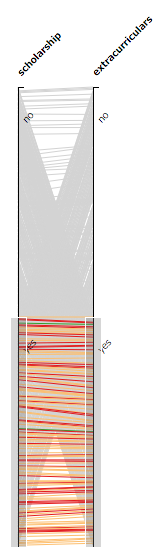
\includegraphics[width=0.2\textwidth]{scholarshipandextracurriculars}
\caption{ The subset of examples that participates in extracurriculars and has scholarship is highlighted. There are slightly more B examples, which are represented by the colored lines, than other grades. }
\label{featureselectiontask1}
\end{figure}

\begin{table}[]
\centering
\begin{tabular}{lc}
\hline
Answers & Frequency \\ \hline
A       & 5       \\
B       & 12         \\
A, B    & 3        \\ \hline
\end{tabular}
\caption{The frequency of the answers. Most participants were able to correctly identify B students as the most frequent target label.}
\label{InterpretFS1}
\end{table}

\subsubsection { Identify Features Separating Two Target Labels }

Second, participants were asked to identify features that distinguish or separate A from F students and those that distinguish B and C students.  To distinguish label u from label v, for each feature, we calculate the ratio of the more frequent label to less frequent label for each feature value. If the ratio is 4 or greater for each of feature value (meaning there is 4 times more of the frequent label than the less frequent label for each feature value), then we say that for the purpose of this task, the feature distinguishes label u from label v.

For A and F students, study time, extra classes, college, and scholarship were distinguishing. For B and C students, only scholarship, college, and study time were distinguishing. We calculated how many distinguishing features participants were able to identify.

Before group B participants started this task, they were first asked which features they thought could be causes or effects of student grades. We noticed that group B participants were likely to identify a distinguishing feature when the feature was previously identified by the participant as being a cause or effect of the target. Participants were relying on their intuitions about what features are important (causal features may be biased as important) to answer these questions. This behavior supports our design of incorporating prior knowledge into the feature selection process.

Participants did not identify all features that distinguish A from F and B from C students. The number of features identified by participants of each group is shown in table \ref{DistinguishingFeatures}. There may be many reasons why participants were not able to identify all distinguishing features. For example, some participants commented that the color associated with a label was visually stronger than that of another label. A subset of the participants utilized the filter for feature value functionality. Most participants utilized class label selection function to filter for the label(s) of interest; they observed the density of colored lines to determine whether a feature distinguishes the two labels/colors. Although there were eleven features and it was feasible to individually assess each feature, participants likely evaluated the entire graph to determine which features clearly separates the two colors. Moreover, for datasets with a larger number of features, we expected a user to be less likely to assess individual features and therefore the user is likely to not identify every distinguishing feature.

A participant commented that they had difficulties identifying patterns in the feature selection graph because the placement of the feature affects the visual. The placement of the feature may obscure the correlation between a feature value and another feature that is placed further away. The participant attempted to figure out what pairs and groups of features distinguish A from F labeled examples by rearranging feature axes; however, they stated they can not exhaust all possible rearrangement of axes. Other participants also commented that it was easier to identify the correlation between feature values when the feature axes were placed next to each other. The placement of the feature axes may be a contributing factor to why a feature was or was not identified as separating two target labels. Although visualization is a more efficient presentation of data, some information may be obscured. This is a ubiquitous challenge in data visualization. We have to sacrifice some clarity and certainty for the efficiency in visual data processing. We recognize that the uncertainty and ambiguity in the visual may increase with the increase in the number of examples and features in the dataset.

The average number of features distinguishing two class labels that the groups of participants identified is presented in table \ref{DistinguishingFeatures}. There is no significant difference between the number of features group A and group B participants are able to identify. However, group B participants behavior supports that causality may be a factor in identifying distinguishing features. Perhaps with a dataset with many more features, it would be more difficult for participants to rely solely on their intuitions about cause and effect relationships and would need help to obtain a complete picture of the causal relationship.

The average amount of time in minutes for participants to answer questions about patterns in the dataset is presented in table \ref{AvgTimeIdentifyPattern}. Participants were able to complete the task in an efficient manner by interpreting and interacting with the visualization. Identifying patterns or correlation between feature values might be more time consuming if the participants were presented with a table of the data or would require knowledge about data science which some of the participants did not have.

\begin{table}[]
\centering
\begin{tabular}{lc}
\hline
Participants & Avg Time (min) \\ \hline
CS (A)         &    10.7  $\pm$ 3.5        \\
Other (A)        &  14.7 $\pm$ 4.6           \\
\textbf{All (A)} & \textbf{12.3 $\pm$ 4.3}    \\ \hline
CS (B)         &    9.0 $\pm$ 5.1        \\
Other (B)        &  11.8  $\pm$ 2.3          \\
\textbf{All (B)} & \textbf{10.3 $\pm$ 3.9}   \\ \hline
\end{tabular}
\caption{The average amount of time for participants to complete the task of identifying patterns}
\label{AvgTimeIdentifyPattern}
\end{table}

\begin{table}[]
\centering
\begin{tabular}{lcc}
\hline
Participants & A and F (4) & B and C (3)\\ \hline
CS (A)       & 2.3 $\pm$ 0.5     & 1.3 $\pm$ 1.0        \\
Other (A)    & 1.8 $\pm$ 1.0      & 1.3  $\pm$ 0.8     \\
\textbf{All (A)} & \textbf{2.1 $\pm$ 0.7}        &  \textbf{1.8 $\pm$ 0.9}       \\ \hline
CS (B)       & 2.5 $\pm$ 0.8      &  1.8 $\pm$ 0.5       \\
Other (B)    & 1.8 $\pm$ 0.8     & 1.5 $\pm$ 0.6      \\
\textbf{All (B)} &   \textbf{2 $\pm$ 0.8} & \textbf{1.7 $\pm$ 0.5}        \\ \hline
\end{tabular}
\caption{The average number of features that were correctly identified as distinguishing A from F and B from C labels.}
\label{DistinguishingFeatures}
\end{table}

\subsection { Analyze Feature Set Metrics }
All the participants were able to determine how many Markov blanket features were covered in the feature selection by reading the Markov Blanket Consistency Chart. In addition, participants were able to determine whether importance features were in the feature selection. A participant explained that they used the Feature Importance Consistency Pie Chart to look at whether ``the green outer boxes corresponding to dark blue boxes", while others cited the rank loss score since higher loss means less consistency.

Some participants noted that feature analysis allowed them to refine their feature selection. A participant commented that when they ``ended up not being very consistent with the causal graph nor with the feature importance selection" which results in them changing their feature selection.

\subsubsection { Compare Feature Set Metrics }
Participants were able to describe the differences in feature analysis metrics between their current feature selection and trial 0, such as the MB score of trial 0 is greater than trial 1 and the rank loss of trial 0 is less than trial 0. However, 8 of the 15 participants did not explain the difference.

\subsubsection { Compare Classifier Performance }
Participants connected or explained a classifier's performance using feature analysis metrics. A participant, who demonstrated a clear understanding of the meaning of the feature metric, related feature metric to the performance of the classifier. They stated that trial 9 had only half of the Markov blanket features hence MB score of 0.5 and may be a reason why trial 9 's feature selection was not as great as trial 0 ’s.
Participants also used feature analysis metrics to help explain why a classifier may perform better than another classifier. For example, a participant explained that trial 1 performed worse than trial 0 because in trial 1 ``the selected features didn't cover all of the contributing factors to grades (hence the low MB coverage score) and weren't the most important". Moreover, a participant commented that trial 1 was ``not very consistent with the causal graph nor the feature importance selection" and attributed those characteristics to the low performance of the classifier.

Some participants commented that they utilized the feature analysis graphs and metrics influence a feature addition or removal.

\subsubsection { Participant Comprehension of Feature Metrics}
The participants demonstrated a good understanding of feature analysis metrics. From the comments on comparing classifiers, participants understand that a lower rank loss, higher MB score, and higher MI score may be the reason for a feature selection that creates a higher performing classifier than another selection. However, not all participants demonstrated that they understand how rank loss score and MB score connected to previously expressed prior knowledge.

Some participants did not understand the concept of Markov blanket coverage. For example, a participant mentioned, “sometimes removing Markov features from a feature selection did not remove the feature from being covered during the feature analysis”. These participants may have thought a feature in the Markov blanket Chart as covered if the feature was in the selected feature set. The concept of coverage was explained in the introductory material but may still be foreign to the participants. The concept can be better explained in the future.

\subsection{ Explore Feature Space}
In this section, we describe how participants in groups A and B explore the feature space and compare and contrast their behaviors.
\begin{table}[]
\centering
\begin{tabular}{lcc}
\hline
                 & CS  \\ \hline
avg \# of trials (A) &  7.3 $\pm$ 3.9        \\
total time (A)       &  13.3 $\pm$ 3.4       \\
\textbf{time per trial (A)}   &  \textbf{2.5 $\pm$ 1.5}         \\ \hline
avg \# of trials (B) &  11  $\pm$ 5.7      \\
total time (B)       &  13.8  $\pm$ 9.0      \\
\texbf{time per trial (B)} &  \textbf{1.3 $\pm$ 0.7}          \\ \hline
\end{tabular}
\caption{The average number of trials completed by group A and B participants and the time spend on the task. }
\label{versionAvsversionB}
\end{table}
\subsubsection { Group A Observations }
Group A participants start with the feature set of target Markov Blanket features in the feature selection. Participants then make minor changes to the Markov blanket feature set. They make elementary changes to the Markov blanket feature set such as adding or removing a feature from the default feature set. Feature additions are more common than feature removals. Initially, participants do not deviate far from the Markov blanket feature set with some exceptions.

Some participants commented that they analyzed the feature analysis before creating the classifier. After a feature was added or removed, they reviewed the feature metrics which influenced whether the change was reversed or not. Group A participants demonstrated that they understand the feature metrics and know how to compare feature metrics of different feature selections. A participant noted that when they saw that a feature selection had a lower MB and MI score than trial 0, the participants changed the feature selection before creating a classifier.
Participants compared their feature selection to trial 0 and aimed to get a better MI score and/or lower rank loss score. Group A also performed fewer trials than group B. Group A was most likely ruling out certain feature sets because of feature metric scores. They were more likely to focus on a subspace of feature sets because of the metrics.

\subsubsection { Group B Observations }
Group B participants were shown an empty set because prior information was not communicated to the system. Before they made feature selection, they were asked which features they thought could be causes or effects of student grades.

Participants relied on their intuition when selecting features and often selected features that they think are causal. When causal discovery is not integrated, participants have to rely on their instincts to figure out which features influence the target. However, participants identified different causal features and initial feature selections varied greatly. By incorporating causality, we can help the user identify causal features that may be predictive.

Moreover, by incorporating causality, participants could identify causal features that they may not have thought about. For example, while participants were able to identify direct causes and effects, they were less equipped to identify indirect influences. GES could provide participants with a complete picture of causal relationships; the visual could help people identify indirect influences to the target that may help build a high performing classifier.

On the other hand, some participants did not start with features that they identify as causal. They started by creating a classifier with a small set of features and added and removed features based on the accuracy of the resulting classifier.

\subsubsection { Group A vs Group B }
Group A participants on average spent more time between trials. Group A participants may be putting in more thought or reasoning about their selected feature set. They may be spending more time between trials because they could evaluate metrics describing the consistency of the feature set. Many participants commented that they review the feature analysis metrics when making feature selections. Some group A participants completed only a few trials in a long stretch of time.

On the other hand, group B participants completed many trials in a similar period of time. Group B participants were more likely to use guesswork when selecting features. Moreover, group B participants did not start with a default feature selection and did not have additional metrics to guide their selection. They rely on their intuition and trial and error. Initial feature sets were usually features they think are causal. Then they remove and add features based on whether the accuracy of the classifier improves.

Trial and error is also a common technique in group A and group B. Participants added or removed features from the selected feature set. Some group A participants did not proceed to create a classifier with that feature set if the metrics are low. For example, most group A participants have 4 or more features in all their trials because the size of their default feature selection is 4 or more and a feature set with less than 4 features would have a low Markov blanket feature score consistency.

On the other hand, group B participants have to verify their intuition and whether they selected predictive features by creating a classifier. As a result, group B participants create more classifiers and also start with a smaller set of selected features.

Another trial and error technique observed in both groups is to remove and add features to the highest performing classifier. 6 (40\%) group A participants and 5 (50\%) group B participants In both groups, the accuracy does not go up continuously. The system stores the iterations of the feature sets and the classifiers and provides graphs to display the progress. Participants were able to compare performances of different iteration. They can then choose to select a previous iteration that performed better and make elementary changes to that feature set. The system is designed for the iterative process of classification and incorporates visuals for comparing performances of different iterations and stores information about previous information. These observations support that the iterative design helps the participants search for high performing classifiers by allowing them to search a subspace of predictive feature sets and comparing feature sets.

We argued that incorporating human’s soft knowledge would be beneficial to the feature selection process. However, we need to be able to leverage their prior knowledge, visual, and analytical capabilities. In version B, although participants were able to recall features they thought may influence student grades, they had to rely mainly on trial and error to test their knowledge. On the other hand, in version A, participants were able to communicate to the system through visuals which features they thought were important. The system and the participants were able to collaboratively build a causal graph; the causal algorithm provided the participant with a possible picture of causal relationships based on suggestions from the participant about which features were important and the participants then correct the graph to more closely reflect their prior knowledge. As a result, group A participants got a more accurate and complete image of the causal relationship. Group A participants also started ahead of group B participants because they started with a set of causal features while group B started with the empty set. Group A had to verify whether the causal features were predictive, while group B had to verify that the feature they thought was important was actually predictive.

Moreover, results from both groups demonstrated the efficiency and usability of the interface and interactions. Participants did not have trouble dragging the feature axes to select features. All participants were able to attempt several trials in less than 30 minutes before deciding on the feature set to predict the target. The amount of time the participants in group A and B spent exploring the feature space is presented in table \ref{versionAvsversionB}.

\subsection { Feature Selection Iterations }
\begin{figure}
    \centering
    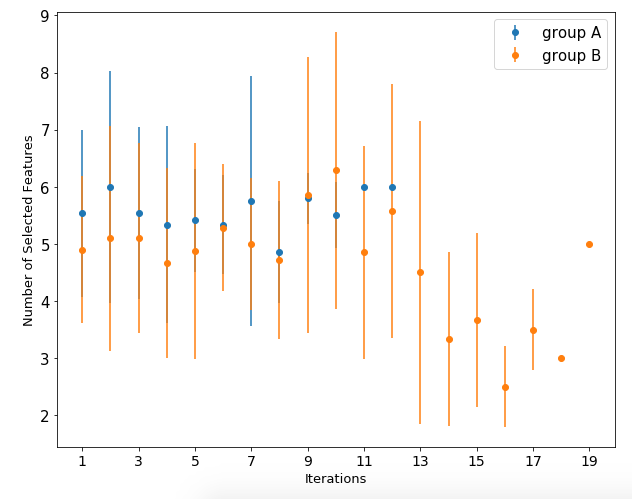
\includegraphics[width=.75\textwidth]{numberofselected}
    \caption{\textbf{Number of Features Selected}. The average number of features selected in each iteration by group A and group B. Group A feature set sizes tend to be bigger than that of Group B in the first 5 trials.  }
    \label{fig:numberofselected}
\end{figure}

\begin{figure}
    \centering
    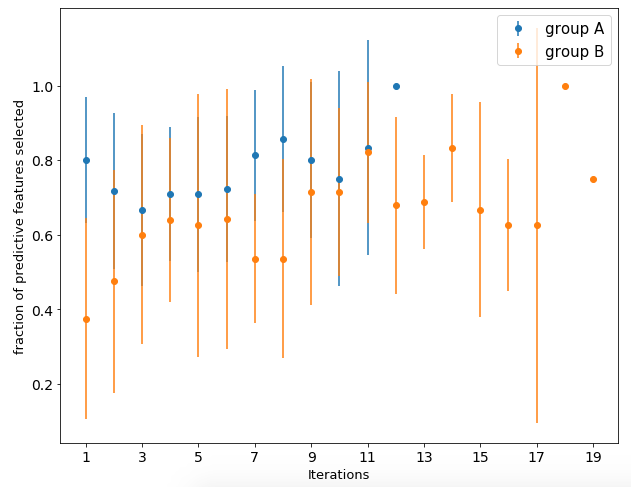
\includegraphics[width=.75\textwidth]{predictivefeaturesselected}
    \caption{\textbf{Fraction of Predictive Features Selected }. The average fraction of the predictive features that was selected in each iteration by group A and group B. On average, group A had more predictive feature in its feature set than group B. }
    \label{fig:predictivefeaturesselected}
\end{figure}

\begin{figure}
    \centering
    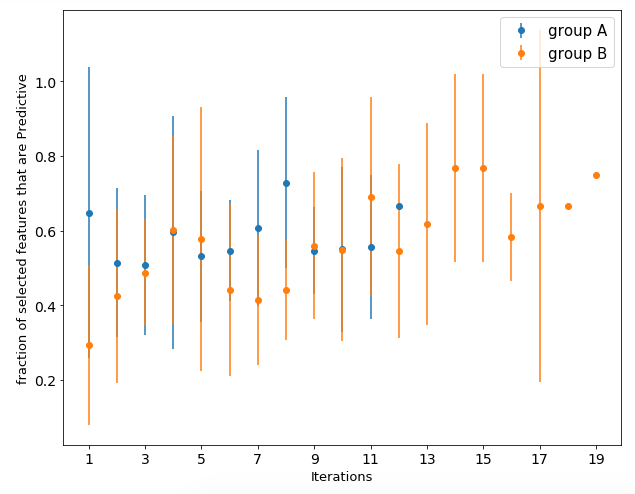
\includegraphics[width=.75\textwidth]{selectedfeaturethatarepredictive}
    \caption{\textbf{Fraction of Selected Features that is Predictive }. The average fraction of the selected feature set that is predictive in each iteration for group A and group B. On average, a bigger fraction of group A's selected feature set is predictive. }
    \label{fig:selectedfeaturethatarepredictive}
\end{figure}

We compare the feature selection behavior of group A and group B. 

The average number of features selected per iteration for group A and group B is plotted in figure \ref{fig:numberofselected}. Group B tend to have smaller feature sets than group A in the first seven trials. This may be because group A started with the set of MB features of the target which can range from 4 to 7 features depending on the causal graph built by the participant. Moreover, the error bars are larger in the first few iterations for group A because some participants removed features while other added features to the set of MB feature. 

The fraction of predictive features selected per iteration by group A and group B is plotted in figure \ref{fig:predictivefeaturesselected}. On average, group A selected more predictive features than group B. Moreover, the error bars for group B are larger which indicates that group B's feature selection behavior varies greater than group A's. 

The fraction of selected features per iteration that are predicted for group A and group B is plotted in figure \ref{fig:selectedfeaturethatarepredictive}. On average, a larger fraction of the selected features is predictive for group A. Moreover, group B starts with a small fraction of the selected features as predictive because group B had to guess and check for predictive features. On the other hand, some of the MB features are predictive so group A starts with a higher fraction of the selected features as predictive. 

\subsection { Effectiveness of Feature Selection }
The irrelevant features in the dataset are motherhasjob, fatherhasjob, age. The causal graph should reveal that these features are irrelevant. Age does not have an edge to or from any of the features which indicates that it is not related to any of the features. Motherhasjob and fatherhasjob are features that do not have a directed path to or from the target variable.

Building the causal graph and expressing feature importance can help reveal predictive features to the participants. For example, study time and college are predictive features and are indicated as more important than the others during the feature importance step.

Furthermore, in the original graph built by GES, the target's Markov blanket contains many predictive features. For example, scholarship, study time, family support, and extra classes are likely to be in the target Markov blanket and are predictive features.

The original graph output by GES could be changed by ranking other features as most important during the expressing feature importance step. From the few participants who ranked other features as most important, the feature they indicated as most important was already in the Markov blanket of the target even if they did not make that indication. Moreover, a participant could change the relationships between the target and a feature in the causal graph which could result in a change in the target's Markov blanket. However, participants did not remove edges to or from the target and more likely to reverse edges which likely adds features to the target's Markov blanket. Therefore, the predictive features were likely to be in the target's Markov blanket when the participant proceeds to the feature selection step.

The feature selection step can also help uncover predictive features. For example, scholarship is predictive and separates both A from F students and B from C students. In addition, study time separates B from C students and is predictive. However, it is noted that not all the participants were able to identify scholarship and/or study time as a distinguishing feature in the previous step; on average, group A and B participants identified about 2 of the 4 features distinguishing A from F and 2 of the 3 features distinguishing B from C.

Relevant feature sets and their testing accuracy are reported in table \ref{relevantFS}.

\begin{table}[]
\centering
\begin{tabular}{ll}
\hline
Feature Sets                                               & Accuracy \\ \hline
extra classes, family support, scholarship, study time (4) & 0.886    \\
extra classes, college, family support, study time (4)     & 0.876    \\ \hline

\end{tabular}
\caption{Predictive feature sets and the accuracy of their classifiers}
\label{relevantFS}
\end{table}

\subsection { Group A Best Feature Selection }

\subsubsection { Likely to include important features }
All but two participants or about 86\%, included study time in their final feature selection as shown in table \ref{RelevantFSBasedOnImportance}. Study time is expressed as the most important feature during the expressing feature importance step. Study time is indicated as an important feature in the Feature Importance Consistency Chart and including it would lower the rank loss score. The most likely reason why study time is in the feature selection is that it was in the Markov blanket of student grade and in the default feature selection. Therefore, the important features indicated by the participant is taken into account when creating the causal graph and making the default feature selection. This helps the participant and the system filter for predictive features.

On the other hand, college was expressed as the second most important feature by all participants. Only 6 participants or about 40\% included college in the final feature selection. It is not in the target's Markov blanket for most of the participants and therefore, not in the default feature selection. This makes it less likely to be in the final feature set.

Most of group B participants also included study time. Most likely because many participants (80\%) thought study time influences student grades. Moreover, many participants (60\%) are able to see that study time separates A from F students or B from C students. Therefore, the feature selection graph can also help participants visually identify predictive features.

\subsubsection { Likely to exclude irrelevant features }
All but 1 participants or about 93\% excluded motherhasjob and fatherhasjob in their final feature set with the exception of a participant who included all the features in their final feature selection, as shown in table \ref{IrrelevantFeatures}. In addition, all participants but two excluded age. Most participants did not include all three features in their trials. This is most likely because they were not apart of the target's Markov blanket and did not have a direct path to or from student grade in the causal graph. Causality is able to help participants filter out irrelevant features.

\subsubsection { Likely to include Markov blanket features }
Group A participants are likely to include Markov blanket features in the final feature set. The final feature set contains may Markov blanket features. On average 75\% of the final feature selection consists of the target's Markov blanket features. At least three of the features in the feature selection are Markov blanket features of the target.

All but three participants include scholarship, which is a predictive feature, in their final feature selection. This is more likely because scholarship is in the default feature selection. Participants also observed that removing scholarship, without replacing it with college, would decrease the performance of the classifier and the Markov blanket score. Of the participants that did not include scholarship, all included college except from one, which shows that they are able to cover scholarship by including college.

Expressing prior information about feature importance and causal relationships help find predictive features.

\begin{table}[]
\centering
\begin{tabular}{lccc}
\hline
Participants & \multicolumn{1}{l}{age} & \multicolumn{1}{l}{mother has job} & \multicolumn{1}{l}{father has job} \\ \hline
group A      & 1 (6.6\%)                &  1 (6.6\%)     &  1 (6.6\%)                                  \\
group B      & 1 (10\%)                 &  1 (10\%)   & 0 (0\%) \\\hline
\end{tabular}
\caption{The number of participants in each group that included the irrelevant features.}
\label{IrrelevantFeatures}
\end{table}

\begin{table}[]
\centering
\begin{tabular}{lccc}
\hline
Participants & \multicolumn{1}{l}{study time} & \multicolumn{1}{l}{college} & job \\ \hline
group A      & 13 (87\%)                      &  9  (60\%) & 13 (87\%)               \\
group B      & 8 (80\%)                       &  6  (60\%) & 3  (30\%)          \\ \hline
\end{tabular}
\caption{The number of participants that included the important and causal feature in their feature selection.}
\label{RelevantFSBasedOnImportance}
\end{table}

\begin{table}[]
\centering
\begin{tabular}{lccc}
\hline
Participants & \multicolumn{1}{l}{scholarship} & \multicolumn{1}{l}{extra classes} & \multicolumn{1}{l}{family support} \\ \hline
group A      & 13 (86\%)   & 6 (40\%)  & 9 (60\%)  \\
group B      & 8 (80\%)     & 6 (60\%)  & 6 (60\%)  \\ \hline
\end{tabular}
\caption{The number of participants that included the feature in their best feature selection.}
\label{RevelantFSBasedOnCausal}
\end{table}

\subsection{Evaluating Feature Sets}
When the participant was asked whether their final selection of features was intuitive, the participant used cause and effect relationships to explain why the features may be predictive of the target. For example, they stated that college and scholarship are predictive because ``college, scholarship are all affected by grade." This shows that users rely on causal relationships they think may exist in the dataset when selecting for features. Furthermore, a participant who has taken a course on machine learning knew to remove redundant features. They stated that ``mother job and father job will influence the family income, and the family income will have an effect on family support. They both have similar influence for grade, so we only necessary pick family support." They understood that the improvements to the classifier will be minimal when adding the features, motherhasjob, and fatherhasjob because their influence on the target is captured in family support.

\subsection { Performance of Classifiers }
The performances of the classifiers created by group A and B are similar. This is because the size of the dataset allows for group B participants to filter for predictive features by trial and error. There are only 11 features and the time to create a classifier is nearly immediate. As a result, group B participants are able to go through many trials and pick out predictive features through trial and error and intuition.

However, we notice differences in the feature selection behaviors of both groups. Group A participants are more likely to spend more time between trials and review the feature analysis metrics before creating a classifier - group A participants averaged 2.5 minutes per trial and group B participants averaged 1.3 minutes per trial. As a result, they create fewer trials and are able to identify a high performing feature set in less trial than group B participants - group A averaged 7.3 trials while group B averaged 11.0 trials. Feature analysis metrics may have helped them identify good sets of features.

Moreover, for a larger dataset with more features, the time to create a classifier will increase. Trial and error will not be a reliable strategy, and the user can not rely on their intuition alone to initially find a good set of features. On the other hand, the user's prior knowledge and complete causal graph help the system and the user focus on a subspace of feature sets and be less likely to go down a rabbit hole. The user can utilize feature analysis metrics to access a feature set before creating a classifier which will only get more time consuming with the complexity of the dataset.

\begin{table}[]
\centering
\begin{tabular}{lcc}
\hline
Participants & \multicolumn{1}{l}{Size of Feature Set} & \multicolumn{1}{l}{Testing Accuracy} \\ \hline
group A      &  5.8 $\pm$ 1.9    &  0.811 $\pm$ 0.008        \\
group B      &  6.0 $\pm$ 2.5  &    0.818 $\pm$ 0.004        \\\hline
\end{tabular}
\caption{Average size of feature size and average accuracy of classifier created from best feature selection}
\label{AccuracyComparison}
\end{table}

\begin{table}[]
\centering
\begin{tabular}{ll}
\hline
Feature Selection Method & Features                                                 \\ \hline
Mutual Information       & college, scholarship, studytime, job, extraclasses       \\
Markov Blanket           & scholarship, familysupport, extraclasses, studytime, job \\ \hline
\end{tabular}
\caption{The features selected by other feature selection methods.}
\label{otherFSmethods}
\end{table}

\begin{table}[]
\centering
\begin{tabular}{lll}
\hline
Feature Selection Method & Feature Set Size & Accuracy \\ \hline
Mutual Information       & 5                & 0.814    \\
Markov Blanket           & 5                & 0.812    \\
group A      &  5.8 $\pm$ 1.9    &  0.811 $\pm$ 0.008        \\
group B      &  6.0 $\pm$ 2.5  &    0.818 $\pm$ 0.004        \\\hline
\end{tabular}
\caption{The feature size and performance of feature sets selected by different feature selection methods.}
\label{otherFSperformance}
\end{table}

\subsubsection { Compare to Other Feature Selection Methods }
We compare the average performance of the feature sets selected by group A and B against the performance of feature sets selected by other non-interactive algorithms, such as mutual information based feature selection and causal feature selection. The features that share the highest amount of information with the target variable are college, scholarship, studytime, job, extraclasses, as reported in table \ref{otherFSmethods}. The accuracy of the classifier using those features is 0.814. In addition, in one causal network generated by GES, the MB of student grade consists of scholarship, familysupport, extraclasses, studytime, job, as shown in figure \ref{fig:Task2} and table \ref{otherFSmethods}; the classifier's accuracy is 0.812. 

Group A and group B did no better and no worse than mutual information based feature selection and causal feature selection. As shown in table \ref{otherFSmethods}, all feature selection methods resulted in classifiers with similar performance. There may be no significant difference in the results because the dataset used the evaluation study may be too trivial and small. The collaborative features selection method did no worse than the other two methods we compared against which shows that our method may help people select predictive features as well as make sense of the predictive feature set. 

\cleardoublepage
\chapter { Conclusion }

In this thesis, we proposed and implemented a collaborative framework for feature selection. By designing visualizations and interactions that facilitate the communication between the user and the machine learning algorithm, we are able to integrate the user's prior knowledge and the user into the feature selection process.

Our feature selection system is a collaborative process that enables the user to encode their prior knowledge. Through interactions with the visualization, the user can visually encode the importance of a feature to the target variable as well as the ranking of the feature according to their importance. The first step of the system is to express and establish prior knowledge and so the system can incorporate additional steps, visuals that represent the user's prior knowledge.

Our implemented feature selection framework integrates causal discovery into the feature selection process and enables the user to integrate their prior knowledge about the causal relationship between features. A causal discovery algorithm incorporates user-provided information about feature importance to build a causal network. Then the user adds, removes, and/or reverse edges in the network to reflect what they previously know about causal relationships in the dataset. Through collaboration facilitated by visualization, the user and system create a causal network that may be more accurate of the underlying data generation mechanisms. The causal network can then help the system and user filter for predictive features.
Moreover, our feature selection step enables the users to dynamically explore the feature space while accessing how consistent the current feature set is to previously express information. By dragging the visual elements representing features, users can quickly build a feature set and efficiently make modifications. The examples are also represented as visual elements rather than described by their feature vector to leverage the user's visual processing power and help them efficiently identify patterns in the dataset. Moreover, a feature analysis page is provided to incorporate the user's prior information. Metrics such as Markov blanket consistency score and rank loss communicates to the user how consistent the current feature set is to their prior knowledge and whether it would possibly be a predictive feature set.

Lastly, our system is designed for the iterative process of classification. Machine learning practitioners have to create a classifier, assess its current performance, make modifications to its inputs such as the feature selection, and then start the process again. We incorporate a performance analysis step that incorporates common and visually effective graphs such as a gradient color coded confusion matrix and the ROC Curve graph. The user can create multiple classifiers from different feature selections. The system keeps track of the previous feature selections and the performances of previous classifiers so that the user can make quick changes to previous feature selections as well as compare the performances of previous classifiers.

After the system was implemented, we designed an evaluation study to access its effectiveness at facilitating collaborative feature selection, interpretability of the visualizations, and its ability to facilitate exploration of feature space. A separate system, version B, that excluded user expressed prior knowledge was created to evaluate the effects of integrating prior knowledge in the feature selection process. A series of tasks were designed to evaluate each part of the process; 15 participants evaluated the full system, while 10 participants evaluated version B.

Our study showed that our system allowed for efficient and effective integration of prior knowledge. Participants communicated feature importance to the system and collaborated with the system to build a possible causal network. Moreover, participants were able to visually process patterns in the datasets; however, some expressed difficulties in identifying patterns. Participants were able to effectively and efficiently explore the feature space; they created many feature selections and classifiers before identifying a set of features for the classification task.

By incorporating and establishing prior knowledge, the participants were able to focus on a subset of the feature space. Although participants using version B and those using the complete system achieved similar performing classifiers, their behavior during the feature selection step differed. Participants using the complete system averaged more time for each classifier because they were utilizing the feature analysis metrics to assess their current feature selection before creating the classifier. Moreover, they started with a default set of features consisting of the features that directly influence the target variable in the causal graph, which made them focus on certain feature sets and make modifications to the default feature set. For more complex datasets, the feature analysis metrics and causal features will guide the user towards a subspace of predictive feature sets.

From the evaluation study, we also observed how the system and our design can be improved. First, two participants commented that the feature selection visual can be difficult to interpret because the orientation of the feature among the other features can either reveal or hide patterns between the features. We hope to investigate and evaluate other methods of displaying the flow of examples from one feature to another; we know that when condensing a lot of information into a visualization some information will be lost or deformed and we seek to minimize that. Second, the color of the examples affect the feature selection visuals, we should use more neutral colors or use colors that relate to the target label. Moreover, we can incorporate other types of prior knowledge.

We can use a different causal discovery algorithm to evaluate whether the causal discovery algorithm makes a difference to the feature selection. Since we observed that prior knowledge is useful for orienting edges in causal networks, we can research and design a more comprehensive framework for interactive causal discovery. Another method to improve on the causal network is to incorporate latent variables, which are variables that can not be measured but can be inferred. We can enable the user to add latent variables and relationships that they inferred to the network. This can improve the understand of the underlying data generating mechanisms. For example, if the user adds a latent variable between a direct cause of the target and the target, then the Markov blanket of the target will change and we can more accurately identify the features that are strongly and weakly relevant to the target. 

Furthermore, we need to incorporate other metrics such as those from filter-based feature selection methods to help user filter for predictive features. We need a metric that communicates the amount of redundant information between pairs of features which can help the user identify redundant information in the feature set.

To sum up, feature selection can greatly benefit from collaboration with humans specifically for integrating prior knowledge.  The proposed feature selection framework integrates effective and efficient visualizations and interactions for establishing prior knowledge and exploring the space of features. With more useful metrics and improvements in the design of visual elements, practitioners can help machine learning algorithms identify a feature set for their classification problem.  The application of interactive machine learning, visual analytics, and novel feature selection techniques have great research potential.

\cleardoublepage
\backmatter
\cleardoublepage
\phantomsection-
\addcontentsline{toc}{chapter}{Bibliography}
\bibliographystyle{IEEEtran}
\bibliography{mybibthesis}
\end{document}

